\documentclass[10pt]{article}
\usepackage[utf8]{inputenc}
\usepackage[T1]{fontenc}
\usepackage{amsmath}
\usepackage{amsfonts}
\usepackage{amssymb}
\usepackage{mhchem}
\usepackage{stmaryrd}
\usepackage{graphicx}
\usepackage[export]{adjustbox}
\graphicspath{ {./images/} }

\title{Introduction }

\author{}
\date{}


\begin{document}
\maketitle
' Flow - To be in constant movement, typically in a single direction. In regards to water, this term typically relates to a volume per unit of time, gallons per minute, cubic feet per second, etc. ${ }^{2}$ Detention time - The theoretical time required to displace the contents of a tank or unit at a given rate of discharge or flow.

\section{Lesson Intent}
This lesson on math basics is intended as a review and introduction to those math concepts believed to be critical and minimum to the "Certified Operator" in an Alaskan community of fewer than 500 population. This does not mean that these are the only math concepts that a competent operator needs in order to solve routine operation and maintenance problems.

\section{Lesson Content}
This lesson on basic math is a review of the principles needed for working with fractions and decimals, rounding numbers, determining the correct number of significant digits, raising numbers to powers, calculating percent, making simple conversions, calculating flow ${ }^{1}$, calculating volume, and calculating detention time ${ }^{2}$.

\section{Basic Equations}
The following is a listing of the basic formulas found in the math section of this text. They have been compiled here for your convenience.

\section{Perimeter/Circumference}
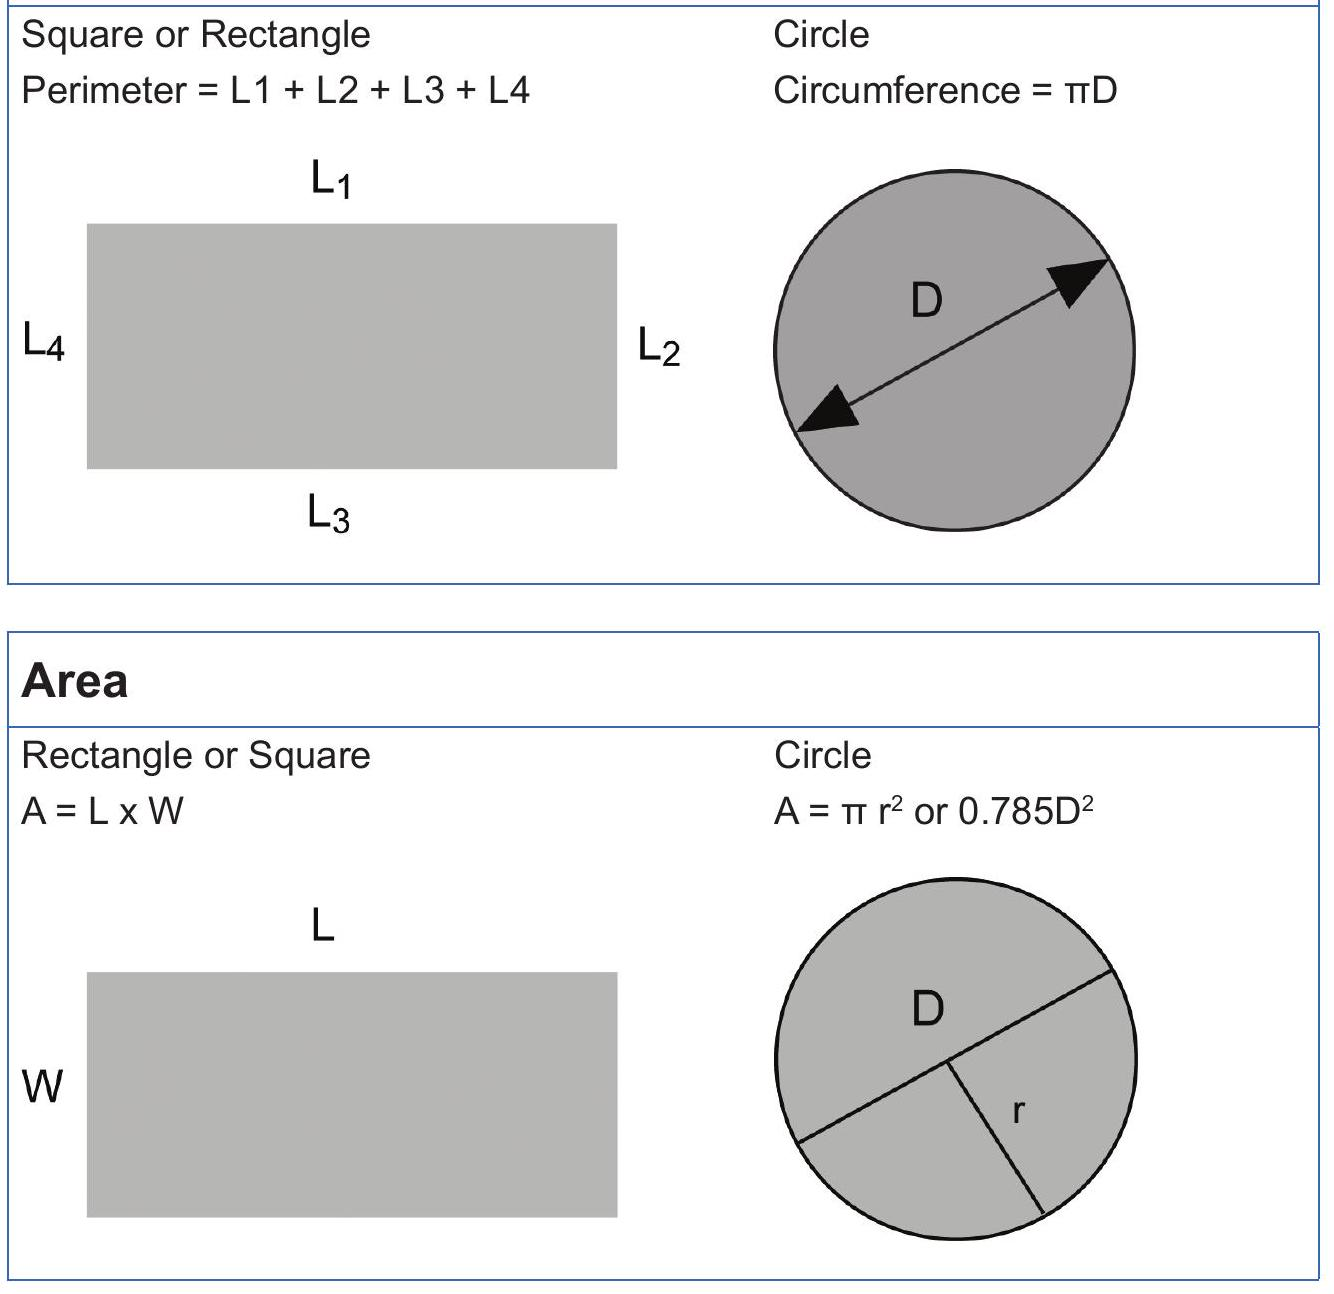
\includegraphics[max width=\textwidth]{2022_09_11_72dbedc910e6e984560cg-01}

\section{Area}
Triangle

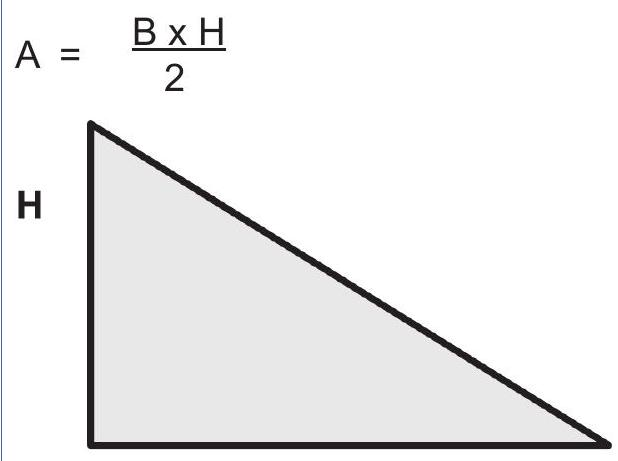
\includegraphics[max width=\textwidth]{2022_09_11_72dbedc910e6e984560cg-02}

B

\section{Other Equations}
\section{Volume}
Rectangle or Square

$V=L \times W \times D$

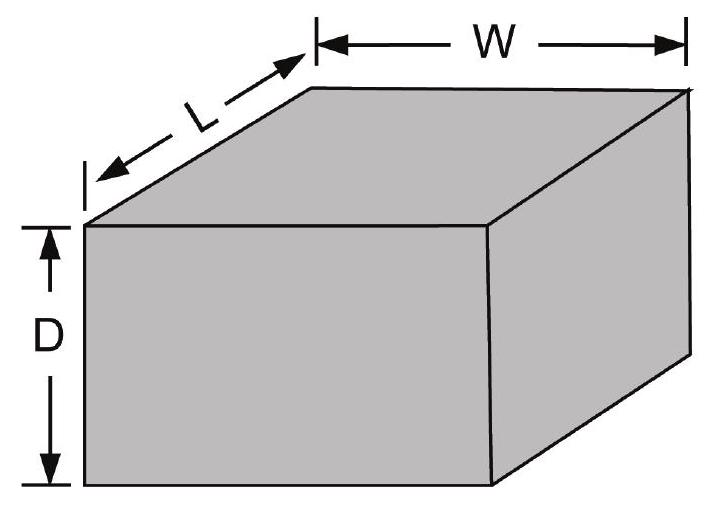
\includegraphics[max width=\textwidth]{2022_09_11_72dbedc910e6e984560cg-02(1)}

Cylinder

$\mathrm{V}=\pi r^{2} \times \mathrm{H}$ or $\mathrm{L}$\\

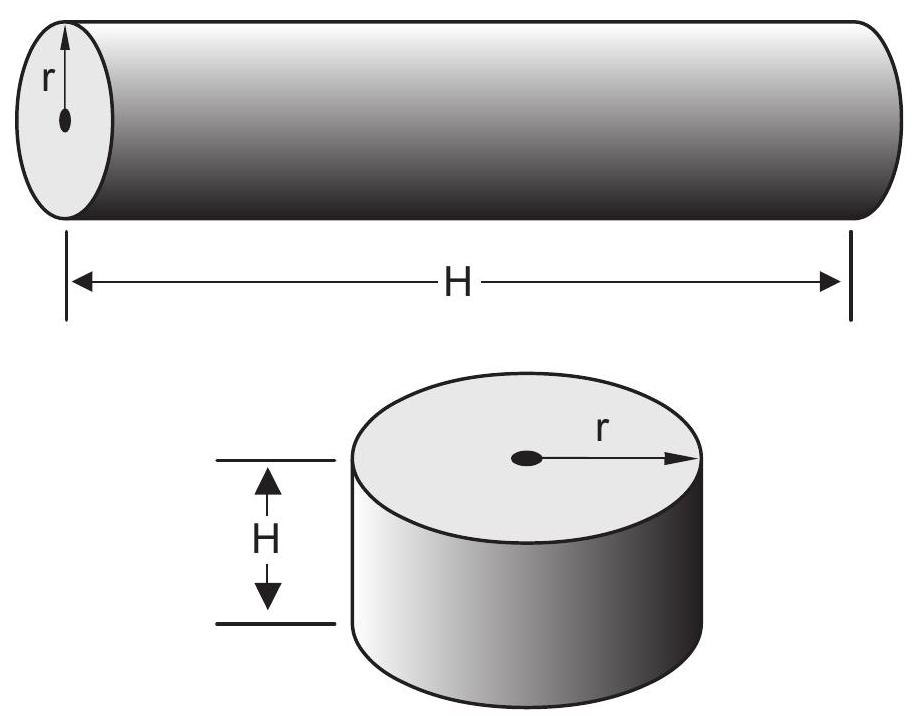
\includegraphics[max width=\textwidth]{2022_09_11_72dbedc910e6e984560cg-02(2)}

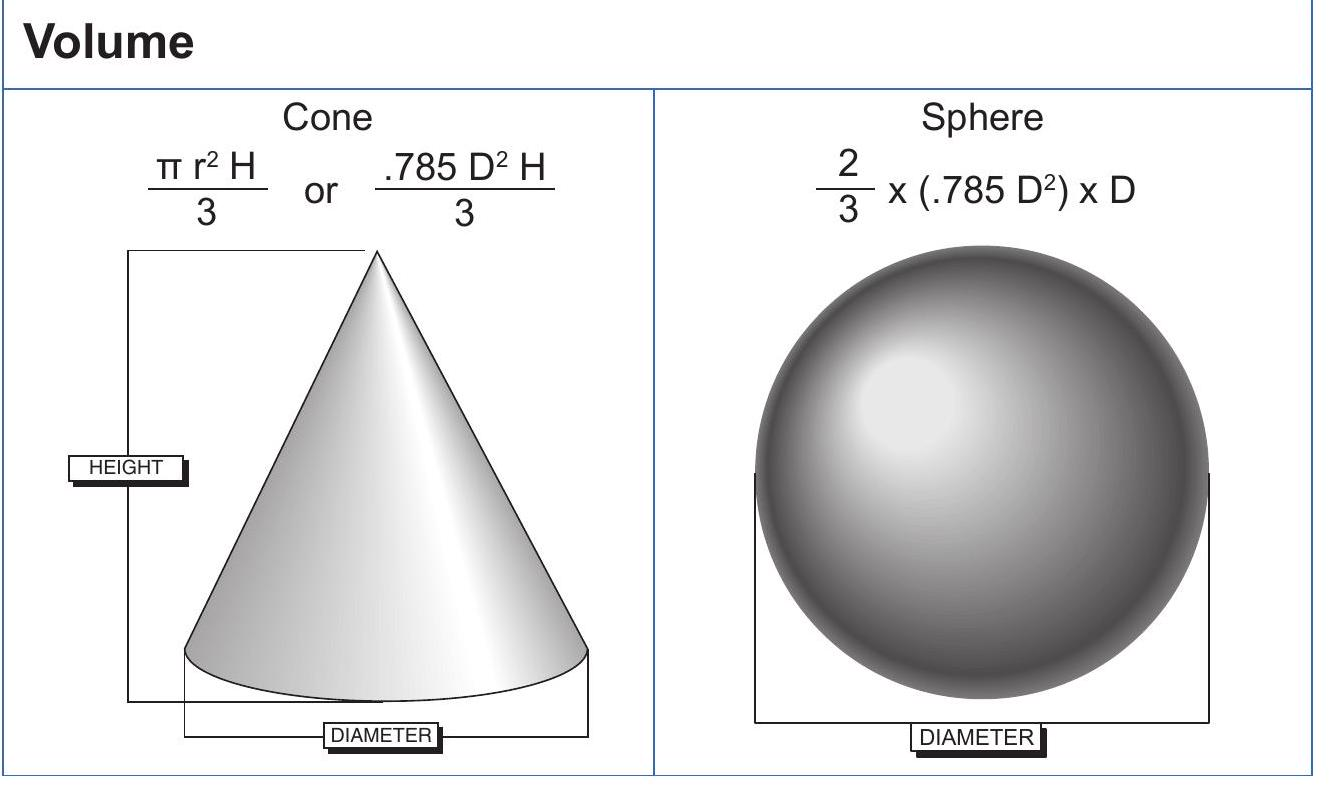
\includegraphics[max width=\textwidth]{2022_09_11_72dbedc910e6e984560cg-03}

\section{Pounds}
$\mathrm{Lbs}=\mathrm{V}, \mathrm{MG} \times 8.34 \mathrm{lbs} / \mathrm{gal} \times$ Conc, $\mathrm{mg} / \mathrm{L}$

Where:

Lbs = pounds

$V=$ flow or volume in millions of gallons

Conc $=$ concentration or dosage in $\mathrm{mg} / \mathrm{L}$

\section{Removal Efficiency}
$$
\frac{\ln -\text { Out }}{\ln } \times 100=\% \text { efficiency }
$$

\section{Pump Efficiency}
$\frac{\text { Output Horsepower }}{\text { Input Horsepower }} \times 100=\%$ efficiency

\section{Weir Overflow Rate}
$$
\text { Weir Overflow Rate }(\mathrm{WO})=\frac{\text { Flow rate in gpd }}{\text { Weir length in feet }}=\mathrm{gal} / \mathrm{day} / \mathrm{ft}
$$

\section{Temperature}
$$
{ }^{\circ} \mathrm{C}=5 / 9\left({ }^{\circ} \mathrm{F}-32^{\circ}\right) \quad{ }^{\circ} \mathrm{F}=\left(9 / 5 x{ }^{\circ} \mathrm{C}\right)+32
$$

\section{Detention Time}
$$
\text { Detention Time }(D T)=\frac{\text { Volume }}{\text { Flow }}
$$

\section{Working with Math}
\section{Steps in Solving Problems}
\section{Introduction}
There are many methods that can be successfully used to solve waterworks problems. We tend to select and adapt problem-solving styles that fit our individual system. If you have selected one or more methods that are beneficial to your style, we suggest that you continue to use what has worked in the past. However, if waterworks problems have frustrated you then we suggest that you consider some version of the following procedure:

\section{Procedure}
\begin{enumerate}
  \item When appropriate, make a drawing of the information in the problem.

  \item Place the data that is available on the drawing.

  \item Ask, "What is the question?"

  \item Write down what you are to find. Sometimes the answer has more than one piece. For instance, you may need to find " $X$ " and then find "Y."

  \item Write down any equation that you are going to need.

  \item Fill in the data in the equation.

  \item Rearrange the equation, if necessary.

  \item Pick up the calculator and make the calculation.

  \item Write down the answer.

\end{enumerate}
\section{Word Problems}
\section{Words to Symbols}
In word problems, certain words can be used to determine the correct math function or meaning. Here are a few of the basic word meaning examples:

Symbols to Words

In writing mathematical formulas or expressions,

\begin{tabular}{|ll|}
\hline
Word & Meaning \\
\hline
of & multiply \\
and & add \\
per & divide \\
less than & subtract \\
\hline
\end{tabular}

symbols are used to indicate an mathematical operation. Here are a few examples:

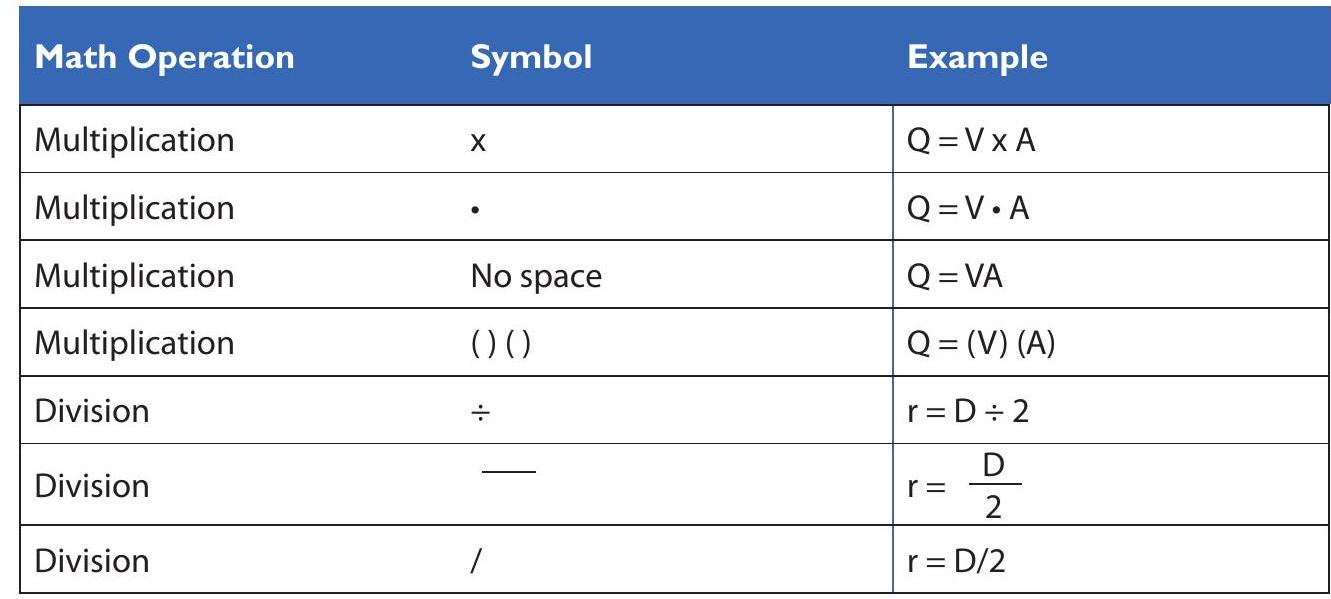
\includegraphics[max width=\textwidth]{2022_09_11_72dbedc910e6e984560cg-04}

3 pi - Greek letter ( $\pi$ ) used as a symbol denoting the ratio of the circumference of a circle to its diameter. ${ }^{4} \mathrm{mg} / \mathrm{L}$ (milligrams per Liter) - A unit of the concentration of a constituent in water. It is $0.001 \mathrm{~g}$ of the constituent in $1,000 \mathrm{ml}$ of water. $\mathrm{mg} / \mathrm{L}$ has replaced the PPM (parts per million) in reporting results in water.

\section{Help with the Calculator}
\section{Introduction}
The calculator has made the solution of waterworks problems much easier and improved our accuracy. At the same time the calculator brings with it its own problems. The following are few hints that may make using the calculator less stressful.

\section{Hint \#1 - Type of Calculator}
The calculator used by a waterworks operator is not a toy; it is a tool like any other tool. As such, it is best to purchase for quality rather than price. Quality will be easier to use and last much longer. A quality calculator used by a waterworks operator should have the following:

\begin{itemize}
  \item The keys should be large enough to allow your fingers to be easily placed on them.

  \item The calculator should have a $\mathbf{p i}^{3}(\pi)$ key. This makes calculating pipe and circular tank volumes much easier.

  \item Solar calculators do not offer the freedom of use that battery calculators offer.

  \item A protective case will add life to the calculator.

  \item The display should allow for 10 characters.

  \item A scientific calculator is more appropriate and useful than a business calculator.

\end{itemize}
\section{Hint \#2 - Read the Book}
The small booklet that comes with the calculator is designed to help you understand the functions of the calculator. You should read and then store the book for easy access. This allows you to use the book to help solve unique problems that show up only on occasion.

\section{Hint \#3 - Division by 2}
One of the common problems confronted by operators is the proper method to solve the following:

\begin{itemize}
  \item One incorrect method that is used is to divide 7 by $0.25$ and then multiply that answer by $8.34$. This will yield an incorrect answer of $233.52 \mathrm{mg} / \mathbf{L}^{4}$.

  \item A second less serious mistake is to multiply $0.25 \times 8.34$ and write the answer down on a piece of scratch paper (2.085). Typically the answer is rounded off to 2 . The rounding reduces the accuracy, and writing the number down is a step that is not necessary.

  \item The CORRECT APPROACH would be to place 7 in the calculator, press the divide key $(\div)$, enter the number $0.25$ and press the divide key $(\div)$ again. Now enter in the number $8.34$, and press the equal key $(=)$. The correct answer of $3.357$ should be displayed. This can be rounded off to $3.4 \mathrm{mg} / \mathrm{L}$. Yes, this is one more character than the correct number of significant digits. This is done not because of accuracy but because the answer is most likely larger than 3 .

\end{itemize}
\section{Math Principles}
\section{Fractions}
Use

With the calculators that are available today, the need to work with fractions is not what it once was. However, the operator is often faced with routine situations that require thinking in fractions and on occasion actually working with fractions. One of the common uses for the rules governing the use of fractions in a math problem is dealing with units of a problem. The unit gpm is actually a fraction gal/min, and $\mathbf{c f s}^{5}$ is actually $\mathrm{ft}^{3} / \mathrm{sec}$. So as you can see, understanding fractions may help you solve other problems.

\section{Components of a Fraction}
A fraction is composed of three items: two numbers and a line. The number on the top is called the numerator, the number on the bottom is called the denominator, and the line in between them means to divide.
$$
\text { Divide } \longrightarrow \frac{3}{4} \quad \begin{aligned}
&\text { Numerator } \\
&\text { Denominator }
\end{aligned}
$$

\section{Principles of Working With Fractions}
Introduction

Like all other math functions, how we deal with fractions is governed by rules or principles. The following is a discussion of 11 principles associated with using fractions.

Same Numerator and Denominator

When the numerator and denominator of a fraction are the same, the fraction can be reduced to 1 . For example:
$$
\frac{4}{4}=1, \frac{24}{24}=1, \frac{8}{8}=1, \frac{12}{12}=1, \frac{125}{125}=1
$$

\section{Whole Numbers to Fractions}
Any whole number can be expressed as a fraction by placing a "1" in the denominator. For example:

2 is the same as $\frac{2}{1}$ and 45 is the same as $\frac{45}{1}$

\section{Adding Fractions}
Only fractions with the same denominator can be added, and only the numerators are added. For example:
$$
\frac{1}{8}+\frac{3}{8}=\frac{4}{8} \text { and }, \frac{6}{32}+\frac{12}{32}=\frac{18}{32}
$$

\section{Subtracting Fractions}
Only fractions with the same denominator can be subtracted, and only the numerators are subtracted. The denominator remains the same. For example:
$$
\frac{7}{8}-\frac{3}{8}=\frac{4}{8} \text { and, } \frac{18}{25}-\frac{6}{25}=\frac{12}{25}
$$

\section{Mixed Numbers}
A fraction combined with a whole number is called a mixed number. For example:
$$
4 \frac{1}{8}, \quad 16 \frac{2}{3}, 8 \frac{3}{4}, 45 \frac{1}{2} \text { and, } 12 \frac{17}{32}
$$
These numbers are read, four and one eighth, sixteen and two thirds, eight and three fourths, forty-five and one half, and twelve and seventeen thirty seconds.

\section{Changing a Fraction}
A fraction can be changed by multiplying the numerator and denominator by the same number. This does not change the value of the fraction, only how it looks. For instance:
$$
\frac{1}{2} \text { is the same as } \frac{1}{2} \times \frac{2}{2} \text { which is } \frac{2}{4}
$$

\section{Simplest Terms}
Fractions should be reduced to their simplest terms. This is accomplished by dividing the numerator and denominator by the same number. The result of this division must leave both the numerator and the denominator as whole numbers. For instance:
$$
\frac{2}{4} \text { is not in its simplest terms, } \frac{1}{2}
$$
The number $2 / 3$ cannot be reduced any further since there is no number that can be divided evenly into the 2 and the 3 .

\section{Practice Problems - Fractions}
\begin{enumerate}
  \item Reduce the following to their simplest terms.\\
A. $4 / 8=$\\
B. $12 / 18=$\\
C. $3 / 4=$\\
D. $6 / 8=$\\
E. $24 / 32=$\\
F. $\quad 9 / 18=$\\
G. $15 / 27=$ Key to Reducing - Even Numbers
\end{enumerate}
When the starting point is not obvious, do the following: if the numerator and denominator are both even numbers $(2,4,6,8,10$, etc.), divide them both by 2 . Continue dividing by 2 until a division will no longer yield a whole number with the numerator and denominator.

Key to Reducing - Odd Numbers

When the numerator and denominator are both odd numbers $(3,5,7,9,11,13,15)$, attempt to divide by three, continue dividing by 3 until a division will no longer yield a whole number with the numerator and denominator. It is obvious that some numbers such as 5, 7, and 11 cannot be divided by 3 and may in fact be in their simplest terms.

\section{Different Denominators}
To add or subtract fractions with different denominators, the denominators must be changed so that all denominators are the same. To find the "common denominator," multiply the denominators together. Then convert each fraction to a new value based on this new common denominator.

For instance, to add $1 / 8$ and $2 / 3$ together:

\begin{enumerate}
  \item Start by multiplying the denominators $8 \times 3=24$.

  \item Change $1 / 8$ to a fraction with 24 as the denominator.

\end{enumerate}
$$
\frac{24}{8}=3, \quad 3 \times 1=3 \text { (the numerator), new fraction is } \frac{3}{24}
$$
Notice that this is the same as $1 / 8$ except $3 / 24$ is not reduced to its simplest terms.

\begin{enumerate}
  \setcounter{enumi}{3}
  \item Change $2 / 3$ to a fraction with 24 as the denominator.
\end{enumerate}
$$
\frac{24}{3}=8, \quad 8 \times 2=16 \text { (the numerator), new fraction is } \frac{16}{24}
$$

\begin{enumerate}
  \setcounter{enumi}{4}
  \item Complete the addition.
\end{enumerate}
$$
\frac{3}{24}+\frac{16}{24}=\frac{19}{24}
$$

\section{Numerator Larger}
Any time the numerator is larger than the denominator, the fraction should be turned into a mixed number. This is accomplished by the following procedure:

\begin{enumerate}
  \item Determine the number of times the denominator can be divided evenly into the numerator. This will be the whole number portion of the mixed number.

  \item Multiply the whole number times the denominator, and subtract from the numerator. This value, the remainder, becomes the numerator of the fraction portion of the mixed number.

\end{enumerate}
$$
\begin{aligned}
&\frac{28}{12}, 28 \text { is divisible by } 12 \text { twice. } 2 \text { is the whole number } \\
&2 \times 12=24 \\
&\frac{28}{12}-\frac{24}{12}=\frac{4}{12} \text { dividing top and bottom by } 4=\frac{1}{3} \\
&\text { New mixed number is } 2 \frac{1}{3}
\end{aligned}
$$
Multiplying Fractions

This is accomplished by the following procedure:

\begin{enumerate}
  \item Multiply the numerators together.

  \item Multiply the denominators together.

  \item Reduce to the simplest terms.

\end{enumerate}
For example: Find the result of multiplying $1 / 8 \times 2 / 3$
$$
\frac{1}{8} \times \frac{2}{3}=\frac{2}{24}, \text { reduced }=\frac{2}{24} \div \frac{2}{2}=\frac{1}{12}
$$
Dividing Fractions

This is accomplished by the following procedure:

\begin{enumerate}
  \item Invert the denominator (turn it upside down).

  \item Multiply and reduce to simplest terms. For example:

  \item Divide $1 / 8$ by $2 / 3$.

\end{enumerate}
$$
\frac{1}{8} \div \frac{2}{3}=\frac{1}{8} \times \frac{3}{2}=\frac{1 \times 3=3}{8 \times 2=16}=\frac{3}{16}
$$
The divide symbol can be $\div$ or $/$ or $-$.

Converting Fractions to Decimals

To convert a fraction to a decimal, simply divide the numerator by the denominator.

Example - Converting Fractions to Decimals
$$
\frac{1}{2}=0.5, \frac{7}{8}=0.875, \frac{7}{16}=0.875, \frac{1}{4}=0.25, \text { and } \frac{2}{3}=0.667
$$
Changing Inches to Feet

To change inches to feet, multiply the number of inches by the conversion $1 / 12$. Example - Changing Inches to Feet

Change 3 inches to feet:

3 in $x \frac{1 \mathrm{ft}}{12 \text { in }}=\frac{3 \text { ift } x 1 \mathrm{ft}}{12 \text { int }}=\frac{3 \mathrm{ft}}{12}=0.25 \mathrm{ft}$

Practice - Changing Inches to Feet

Change the following to feet:

2 inches, 4 inches, 6 inches, 8 inches

$\frac{2}{12}=0.167$ feet

$\frac{4}{12}=0.33$ feet

$\frac{6}{12}=0.5$ feet

$\frac{8}{12}=0.667$ feet

\section{Decimals}
The Components

A decimal is composed of two sets of numbers: the numbers to the left of the decimal are whole numbers, and numbers to the right of the decimal are parts of whole numbers, a fraction of a number.

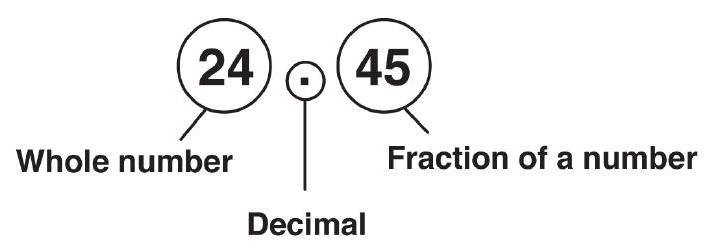
\includegraphics[max width=\textwidth]{2022_09_11_72dbedc910e6e984560cg-10}

\section{Fraction Component}
The term used to express the fraction component is dependent on the number of characters to the right of the decimal.

\begin{itemize}
  \item The first character after the decimal point is tenths: $0.1$ - tenths

  \item The second character is hundredths: $0.01$ - hundredths

  \item The third character is thousandths: $0.001$ - thousandths

\end{itemize}
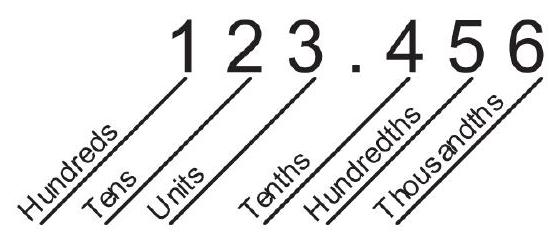
\includegraphics[max width=\textwidth]{2022_09_11_72dbedc910e6e984560cg-10(1)}

\section{Principles}
Calculators

With today's use of calculators, we seldom need the rules for handling decimals. As a result, when we need to make a computation manually, we often cannot remember the basic rules. Therefore, this brief review is provided.

Number Less Than One

When a number is less than one and is expressed as a decimal, place a "0" (zero) to the left of the decimal. This makes it clear that the number is less than one. For instance $0.25$ is much clearer than 25 .

\section{Subtraction}
When subtracting decimals, simply line up the numbers at the decimal, and subtract.

For example:

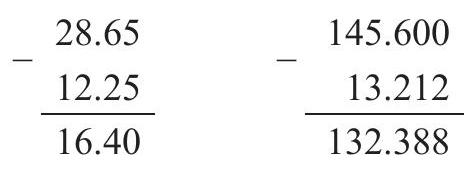
\includegraphics[max width=\textwidth]{2022_09_11_72dbedc910e6e984560cg-11}

\section{Addition}
To add numbers with a decimal, use the same rules as subtraction: line up the numbers on the decimal, and add.
$$
\begin{array}{r}
28.65 \\
12.25 \\
\hline 40.90
\end{array}+\begin{array}{r}
145.600 \\
13.212 \\
\hline 158.812
\end{array}
$$

\section{Multiplication}
To multiply two or more numbers containing decimals, follow these few basic steps:

\begin{enumerate}
  \item Multiply the numbers as whole numbers. Do not worry about the decimals.

  \item Write down the answer.

  \item Count the total number of digits (numbers) to the right of the decimal in all of the numbers being multiplied.

  \item To place the decimal in the answer, count from the right to the left the number of digits counted in the previous step.

\end{enumerate}
\section{Example - Multiplication}
Multiplying $3.04$ x $8.6$ yields the number 26144 .

There are a total of three digits to the right of the decimal point ( 2 for the number $3.04$ and 1 for the number 8.6). Therefore, the decimal point should be placed three places to the left from the right of the last 4 .

\section{Division}
To divide a number by a number containing a decimal, the divisor must be made into a whole number by moving the decimal point to the right until you have a whole number.

\begin{enumerate}
  \item Count the number of places the decimal needed to be moved.

  \item Move the decimal in the dividend by the same number of places.

  \item Make the division.

\end{enumerate}
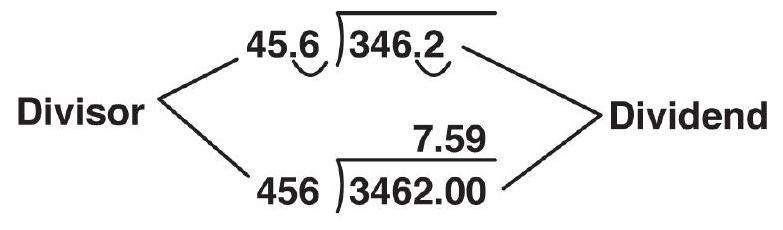
\includegraphics[max width=\textwidth]{2022_09_11_72dbedc910e6e984560cg-12}

Using the Calculator

With today's calculators, this problem would simply be set up as follows:
$$
\frac{346.2}{45.6}=7.59
$$

\section{Rounding}
Why Round?

Numbers are rounded to reduce the number of digits to the right of the decimal point. This is for convenience, not accuracy.

\section{Process of Rounding}
\begin{enumerate}
  \item Start by deciding how many places you want to the right of the decimal. Remember this is done for convenience.

  \item If the number to the right of the last number that you wish to report is 5 or greater than 5 , increase the size of the last number by 1 .

  \item If the number to the right of the last number that you wish to report is less than 5 , the size of the last number remains the same.

\end{enumerate}
\section{Example 1 - Rounding}
A calculation has just been completed, and the answer is $24.55836$. A decision is made to have two places to the right of the decimal. Two places takes you to $25.55$. The next number is "8." Therefore, the last five is rounded up to a six. The number is $24.56$.

\section{Example 2 - Rounding}
A calculation has just been completed, and the answer is $24.55436$. A decision is made to have two places to the right of the decimal. Two places takes you to $25.55$. The next number is "4." Therefore, all of the numbers to the right of the $.55$ are dropped. The reported number is $24.55$.

\section{Practice Problems - Rounding}
\begin{enumerate}
  \item Round the following to the nearest hundredths (the second place after the decimal).\\
A. $2.4568$\\
B. $27.2534$\\
C. $128.2111$\\
D. $364.8762$\\
E. $354.777777$\\
F. $34.666666$\\
G. $67.33333$

  \item Round the following to the nearest tenths (the first place after the decimal).\\
A. $2.4568$\\
B. $27.2534$\\
C. $128.2111$\\
D. $364.8762$\\
E. $354.777777$\\
F. $34.666666$\\
G. $67.33333$

\end{enumerate}
\section{Determining Significant Digits}
\section{The Concept}
Significant digits are related to rounding. We use the concept to determine the direction to round a number. The basic idea is that no answer can be more accurate than the least accurate piece of data used to calculate the answer.

\section{Process}
There are several rules used to determine whether a digit is significant:

\begin{enumerate}
  \item Non-zero digits are significant. ie. numbers $1-9$

  \item Zero's appearing between non-zero digits are significant. ie. 103, 24000.2, $10.7$

  \item Zero's appearing to the right of a decimal ar significant. ie. $12.00,8.3400,0.020$

  \item Zero's appearing at the beginning of a number are NOT significant. ie $\mathbf{0 . 4}$

\end{enumerate}
\section{Practice Problems - Significant Digits}
For addition and subtraction the process involves two steps:

\begin{enumerate}
  \item Determine the number of decimal places in the least accurate piece of data.

  \item Round off the answer to theis position.

\end{enumerate}
Example - Significant Digits

The following calculation was made: The least accurate piece of data is number 12.27. As $12.27$ has only 2 decimal places the sum can have only 2 decimal places as well. The correct answer is 57.55.

\begin{enumerate}
  \item Round the following answers off to the most significant digit.
\end{enumerate}
\begin{tabular}{|l|l|l|}
\hline
 & Problem & Accurate Answer \\
\hline
A. & $25.1+26.43=51.53$ &  \\
\hline
B. & $128.456-121.4=7.056$ &  \\
\hline
C. & $85-7.92432=77.07568$ &  \\
\hline
D. & $8.564+5=13.564$ &  \\
\hline
\end{tabular}

\section{For multiplication and division the process involves two steps:}
\begin{enumerate}
  \item Determine the number of significant figures each number has.

  \item Round the final answer to the number with the least significant digits.

\end{enumerate}
\section{Example - Multiplication and Division with Significant Digits}
The following calculation was made:

$53.2 \times 128.64=6,843.648$

In the above problem, $53.2$ has 3 significant figures and $128.64$ has 5 . The multiplication/division rule says the answer should be rounded to the number with the least number of significant digits; in this case three (53.2). So the correct answer is 6,840 .

$2 .$

\begin{tabular}{|l|l|l|}
\hline
 & Problem & Accurate Answer \\
\hline
A. & $26.34 \times 124.34567=3,275.26495$ &  \\
\hline
B. & $23.58 \times 34.251=807.63858$ &  \\
\hline
C. & $12,453 / 13.9=895.8992805755$ &  \\
\hline
D. & $12,457.92 \times 3=37,373.76$ &  \\
\hline
\end{tabular}

${ }^{6}$ Area - The extent of a surface, measured by the number of squares of equal size it contains.

${ }^{7}$ Cubic Feet - A measurement of volume in the number of cubes that are one foot on a side.

\section{Working with Powers}
Principle

Powers are used to identify area ${ }^{6}$, as in square feet, and volume as in cubic feet ${ }^{7}$. Powers can also be used to indicate that a number should be squared, cubed, etc. This later designation is the number of times a number must be multiplied by itself.

Example - Powers

We could find these two numbers:

$4^{2}$ or $4 \mathrm{ft}^{2}$

The number $4^{2}$ means $4 \times 4=16$.

The number $4 \mathrm{ft}^{2}$ means four square feet, an area $2 \mathrm{ft} \times 2 \mathrm{ft}$.

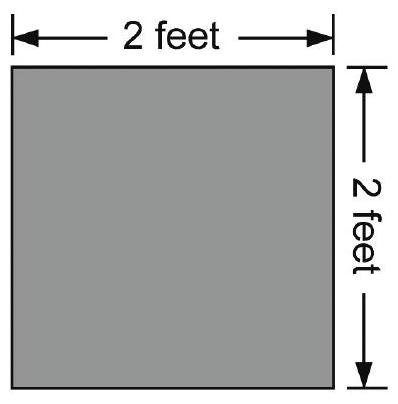
\includegraphics[max width=\textwidth]{2022_09_11_72dbedc910e6e984560cg-15}

Or we might see these two numbers $4^{3}$ or $4 \mathrm{ft}^{3}$.

The number $4^{3}$ means $4 \times 4 \times 4=64$.

The number $4 \mathrm{ft}^{3}$ means 4 cubic feet, a block $2 \mathrm{ft} \times 2 \mathrm{ft} \times 1$ foot deep.

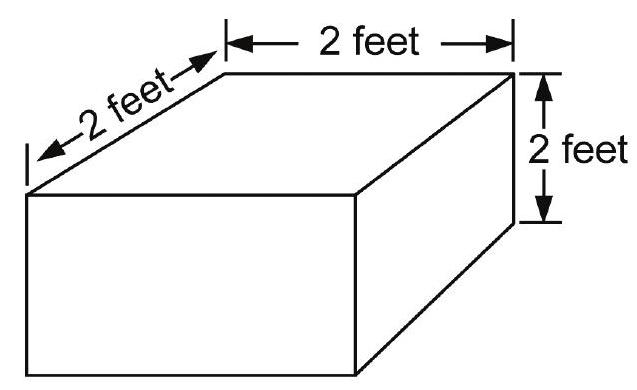
\includegraphics[max width=\textwidth]{2022_09_11_72dbedc910e6e984560cg-15(1)}

\section{Finding Averages}
Use

Finding an average $^{8}$ of a series of numbers is accomplished by adding the num-

${ }^{8}$ Average - An arithmetic mean. The value is arrived at by adding the quantities in a series and dividing the total by the number in the series. bers and dividing by the number of numbers in the group. This is an activity that is required on the monthly report for chlorine, fluoride, and turbidity readings. The average for the month is commonly figured on all chemicals added, and on most test results. Example 1 - Averages

Find the average of the following series of numbers: $12,8,6,21,4,5$, 9 , and 12 . Adding the numbers together we get 77 . There are 8 numbers in this set. Divide 77 by 8 .

$\frac{77}{8}=9.6$ is the average of the set

Example 2 - Averages

Here is a series of daily turbidities. Obtain the average for them.
$$
0.3,0.4,0.3,0.1,0.8
$$
The total is 1.9. There are 5 numbers in the set. Therefore:
$$
\frac{1.9}{5}=0.38, \text { rounding off }=0.4
$$

\section{Practice Problem - Averages}
\begin{enumerate}
  \item Find the average of the following set of numbers:
\end{enumerate}
$$
\begin{aligned}
&0.2 \\
&0.2 \\
&0.1 \\
&0.3 \\
&0.2 \\
&0.4 \\
&0.6 \\
&0.1 \\
&0.3
\end{aligned}
$$

\section{Equations}
\section{Description}
An equation is a symbolic representation of how to combine certain information in order to obtain the proper result. Equations are written using letters and symbols to represent unknown or standard values.

Use

Equations (also called formulas) are used by operators to solve a wide variety of problems associated with treatment and collection. In fact, most operators use formulas without thinking about them to solve routine problems. For instance, to determine the perimeter or distance around a building requires using a formula.

\section{Example 1 - Equations}
The equation for determining the perimeter of a triangle is $\mathrm{P}=\mathrm{a}+\mathrm{b}+\mathrm{c}$. $\mathrm{P}$ is the letter used to designate the perimeter and $\mathrm{a}, \mathrm{b}$, and $\mathrm{c}$ are used to identify the lengths of the sides. The mathematical symbols $(=)$ and $(+)$ tell the user what math functions are to be carried out. This formula says to add the lengths of all of the sides to obtain the perimeter.

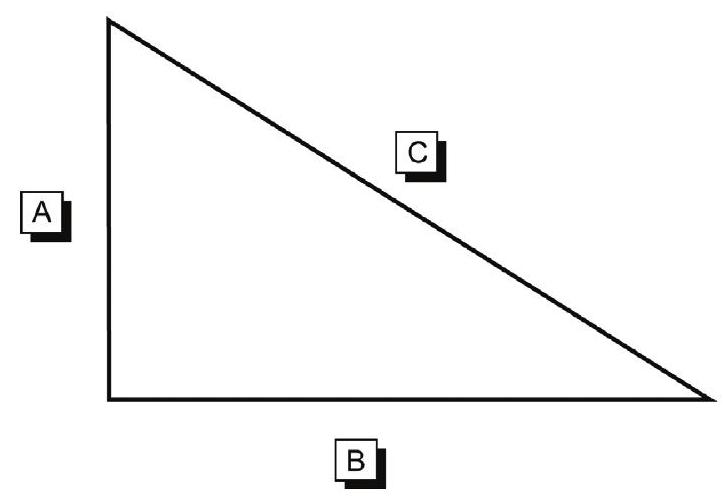
\includegraphics[max width=\textwidth]{2022_09_11_72dbedc910e6e984560cg-17}

\section{Example 2 - Equations}
In the example below, the numbers $3^{\prime}, 4^{\prime}$, and $5^{\prime}$ have been substituted for the letters a, b, and c. To solve the equation substitute the numbers for the appropriate letters, $a=3^{\prime}, b=4^{\prime}$, and $\quad \mathrm{c}=5^{\prime}$. Now add the three together to obtain a perimeter of $12^{\prime}$. The distance around this triangle is 12 feet.

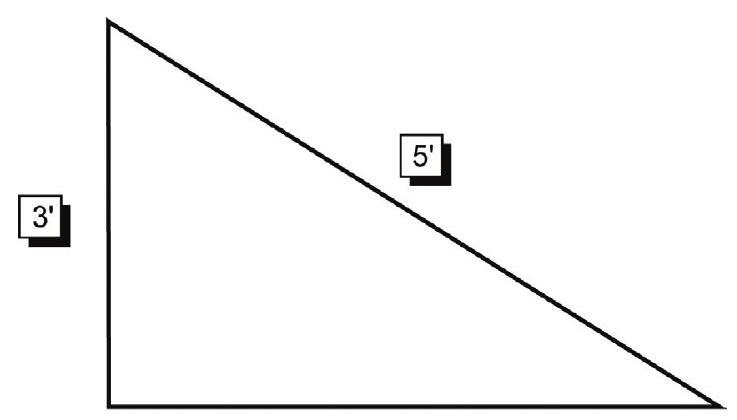
\includegraphics[max width=\textwidth]{2022_09_11_72dbedc910e6e984560cg-17(1)}

$4^{\prime}$

\section{Works on All Triangles}
This equation will work for all triangles, regardless of the lengths of their sides.

\section{Formulas with Symbols}
Some equations such as the one for the area of a circle $\left(\mathrm{A}=\pi \mathrm{r}^{2}\right)$ use symbols. The symbol $\pi$ (pi) is used to represent a constant: 3.14. This is done in equations to simplify the writing of the equation.

\section{Listing of Formulas}
A listing of common equations used in water/wastewater systems can be found at the end of this chapter. In addition, equations are used in most of the other sections of this chapter.

\section{Rearranging Equations}
Types of Equations

The equations that are commonly used in water math are called linear equations (follow a straight line). To be successful in solving math problems, an operator must be able to solve a linear equation with one unknown (perimeter of a triangle, pounds formula, area of a circle are all examples of this type of equation).

\section{Why Rearrange?}
To solve a problem, an operator is often required to solve the equation for a component that is not normally part of the solution. For instance, the perimeter and the length of two sides of a triangle may be known, and you wish to solve for the length of the third side.

\section{Two Sides}
Equations have two sides that are separated by the equal sign $(=)$. To solve an equation, there must be only one unknown and the unknown must be on one side of the equation by itself.

\section{Rearranging Equations with Addition and Subtraction}
Rule

The rule of equality must be maintained! Thus, if you subtract a value from the right side of the equal sign, you must subtract the same value from the left side of the equal sign. The is true for adding, dividing, and multiplying.

\section{Example - Addition and Subtraction}
Solve the equation $12=3+b+5$

The first step is to rearrange the equation so that the unknown is on one side of the equation by itself. This is accomplished by subtracting 3 and 5 from both sides of the equation.

$12-3-5=3+b+5-3-5$

On the right side of the equation $3-3=0$ and $5-5=0$

The resulting new equation would look like this:

$12-3-5=\mathrm{b}$

The last step is to do the math. That is, subtract 3 and 5 from 12. The result is: $4=b$

\section{Rearranging Equations with Multiplication and Division}
\section{Process}
To solve for an unknown value in an equation using multiplication or division, move the unknown value to one side of the equation by itself.

\section{Top and Bottom}
As stated above, an equation has two sides. A multiplication and division equation also has a top and bottom that are separated by a division line. When the equation is just multiplication, the division line is not shown and all of the items are above the line. Rule

To move an item from one side of an equation to the other in a multiplication or division equation, the item is moved from the top of one side to the bottom of the other or from the bottom of one side to the top of the other.

\section{Summary}
To state it another way, if the item that is being moved is on top of the equation, then it must be placed below when moved. If an item is below in the equation, then it must be placed above when it is moved.

\section{Example 1 - Multiplication and Division}
Solve this equation for $\mathrm{V}$ :
$$
254=\mathrm{V} \times 8.34 \times 35
$$
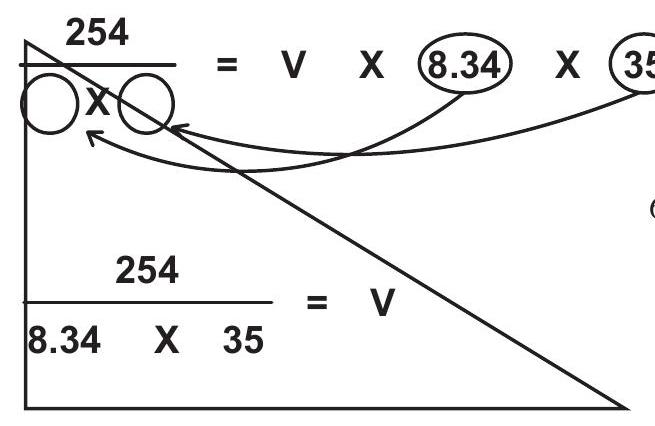
\includegraphics[max width=\textwidth]{2022_09_11_72dbedc910e6e984560cg-19}

Result:

$V=0.87$

Example 2 - Multiplication and Division

Solve for $\mathrm{X}$ in the following equation:
$$
6=\frac{x}{10}
$$
Step 1 - Rearrange the equation by multiplying both sides by 10 .

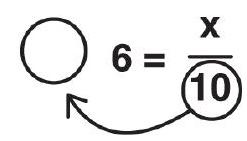
\includegraphics[max width=\textwidth]{2022_09_11_72dbedc910e6e984560cg-19(1)}
$$
10 \times 6=X
$$
Step 2 - Solve the equation.
$$
60=\mathrm{X}
$$

\section{Special Note}
Many equations are written without the use of the multiplication sign. For instance, $\mathrm{A}=\pi \mathrm{r}^{2}$ and $\mathrm{C}=\pi \mathrm{D}$.

$\pi \mathrm{r}^{2}$ is the same as $\pi \times \mathrm{r}^{2}$, or pi times $\mathrm{r}^{2}$.

Also, $\pi\left(r^{2}\right)$ is the same as $\pi \times\left(r^{2}\right)$ or pi times $r^{2}$.

\section{Equation Problems}
Example 1 - Equation Problems

A triangle has a perimeter of 24', the length of the bottom is 8 ', and the length of the left side is 6 '. What is the length of the long side?

Step 1 - Draw a diagram of the triangle.

Step 2 - Place the known values on the diagram.

Step 3 - Write the equation.

$\mathrm{P}=\mathrm{a}+\mathrm{b}+\mathrm{c}$

Step 4 - Fill in the known values in the equation.

$24^{\prime}=6^{\prime}+8^{\prime}+c$

Step 4 - Subtract 6' and $8^{\prime}$ from both sides of the equation.

$24^{\prime}-6^{\prime}-8^{\prime}=\mathrm{c}$

Step 5 - Solve the equation.

$10^{\prime}=\mathrm{c}$ Example 2 - Equation Problems

Find the diameter of a pipe with a circumference of $187 / 8$ inches.

Step 1 - Draw a diagram of the pipe.

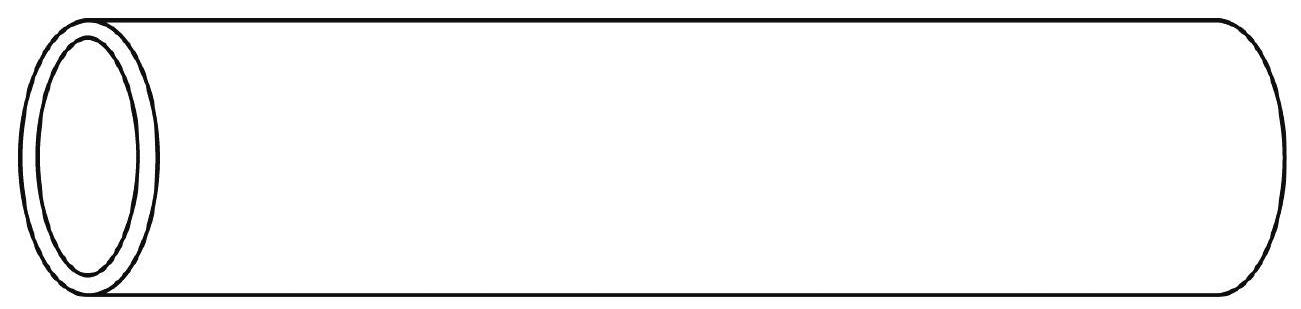
\includegraphics[max width=\textwidth]{2022_09_11_72dbedc910e6e984560cg-21}

Step 2 - Place the known values on the diagram.

Circumference $=187 / 8 "$\\

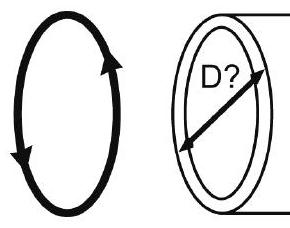
\includegraphics[max width=\textwidth]{2022_09_11_72dbedc910e6e984560cg-21(1)}

Step 3 - Make any obvious conversions.

The circumference is given in inches and fractions of inches. This must be converted to a decimal before proceeding.

$187 / 8^{\prime \prime}=18.875 "$

Step 4 - Select an equation.

$\mathrm{C}=\pi \mathrm{D}$

Step 5 - Fill in the known values.

$18.75 "=\pi \mathrm{D}$

Step 6 - Divide both sides of the equation by pi.

$\frac{18.75^{\prime \prime}}{\pi}=\mathrm{D}$

Step 7 - Solve the equation.

$6 "=\mathrm{D}$ Example 3 - Equation Problems

Find the diameter of a settling basin with a surface area of $1257 \mathrm{ft}^{2}$.

Step 1 - Draw a diagram of the clarifier.

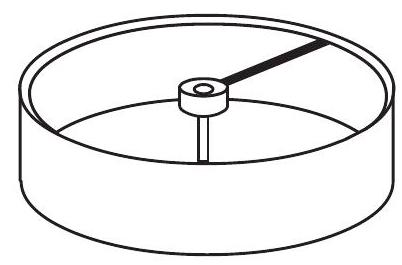
\includegraphics[max width=\textwidth]{2022_09_11_72dbedc910e6e984560cg-22}

Step 2 - Place the known values on the diagram.

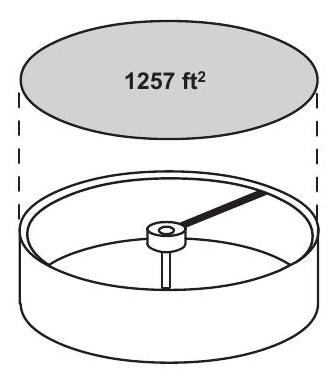
\includegraphics[max width=\textwidth]{2022_09_11_72dbedc910e6e984560cg-22(1)}

Step 3 - Select an equation.

$A=\pi r^{2}$

Step 4 - Fill in the known values.

$1257 \mathrm{ft}^{2}=\pi \mathrm{r}^{2}$

Step 5 - Divide both sides of the equation by pi $(\pi)$.

This rearrangement will require two steps. The second step is to change the $\mathrm{r}^{2}$ to $\mathrm{r}$. This is accomplished by finding the square root of all of the values on both sides of the equation.

$\sqrt{\frac{1257 f t}{2}}=\mathrm{r}$

20 feet $=r$

Step 6 - Determine the diameter from the radius.

Since the radius is one half of the diameter this value must be multiplied by 2 .

$2 \times 20 \mathrm{ft}=40 \mathrm{ft}-$ the diameter of the clarifier Example 4 - Equation Problems

A chlorine contact chamber holds 2700 gallons. It is desired to have a contact time of 30 minutes in the chamber. What is the maximum flow rate that can pass through this chamber at this detention time.

Step 1 - Draw a diagram of the situation.

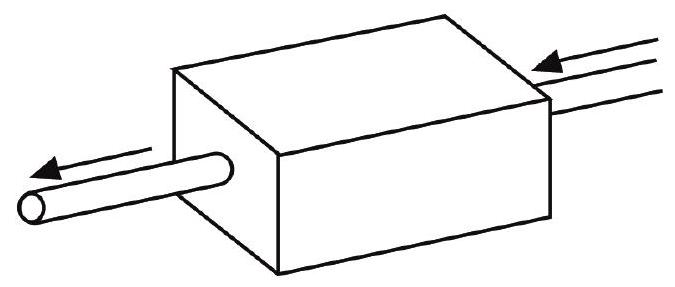
\includegraphics[max width=\textwidth]{2022_09_11_72dbedc910e6e984560cg-23}

Step 2 - Place the unknown values on the diagram.

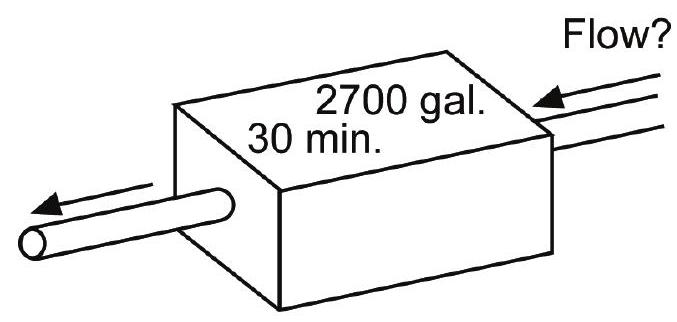
\includegraphics[max width=\textwidth]{2022_09_11_72dbedc910e6e984560cg-23(1)}

Step 3 - Select an equation.
$$
\mathrm{DT}=\frac{\text { Volume }}{\text { Flow }}
$$
Step 4 - Place the known values in the equation.
$$
30 \min =\frac{2,700 \text { gal }}{\text { gpm }}
$$
Step 5 - Divide both sides of the equation by 30 minutes.
$$
\mathrm{gpm}=\frac{2,700 \mathrm{gal}}{30 \mathrm{~min}}
$$
Step 6 - Solve the equation.

$\operatorname{gpm}=90 \mathrm{gpm}$

\section{Practice Problems - Formulas}
\begin{enumerate}
  \item Find the diameter of a settling basin that has a circumference of 126 feet.

  \item Find the diameter of a pipe that has a circumference of $129 / 16 " .$ 3. Find the diameter of a settling basin that has a surface area of $113 \mathrm{ft}^{2}$.

  \item Find the diameter of a storage tank that has a surface area of $314 \mathrm{ft}^{2}$.

  \item The detention time in a chlorine contact chamber is 42 minutes. If the chamber holds 3200 gallons, what is the flow rate in gpm? ${ }^{9}$ Circumference - The perimeter of a circle. ${ }^{10}$ Rectangle - A four-sided figure with four right angles.

  \item A clearwell has a detention time of 2 hours. What is the flow rate in gpm if the clearwell holds 8000 gallons?

  \item A rectangular settling basin has a weir length of 10 feet. What is the weir overflow rate when the flow is $80,000 \mathrm{gpd}$ ?

\end{enumerate}
\section{Finding Perimeter/Circumference}
Units

The perimeter is the total distance or length around an object, like a parcel of land, a building, or a box. Circumference ${ }^{9}$ is the distance around a circle. Distance is a linear measurement, and therefore the standard units for linear measurements are used. Typical samples would be inches, feet, miles, etc.

Formula for a Rectangle

The perimeter of a rectangle ${ }^{10}$ is obtained by adding the lengths of the four sides. 11 Diameter - The distance across a circle. A straight line passing through the center of a circle. Formula for a Circle

The circumference of a circle is found by multiplying pi $(\pi)$ times the diameter ${ }^{11}$.

$\mathrm{C}=\pi \times \mathrm{D}$

Where:
$$
\begin{array}{ll}
\mathrm{C}=\text { Circumference } & \pi=\text { Greek letter pi } \\
\mathrm{D}=\text { Diameter } & \pi=3.1416
\end{array}
$$

\section{Perimeter/Circumference}
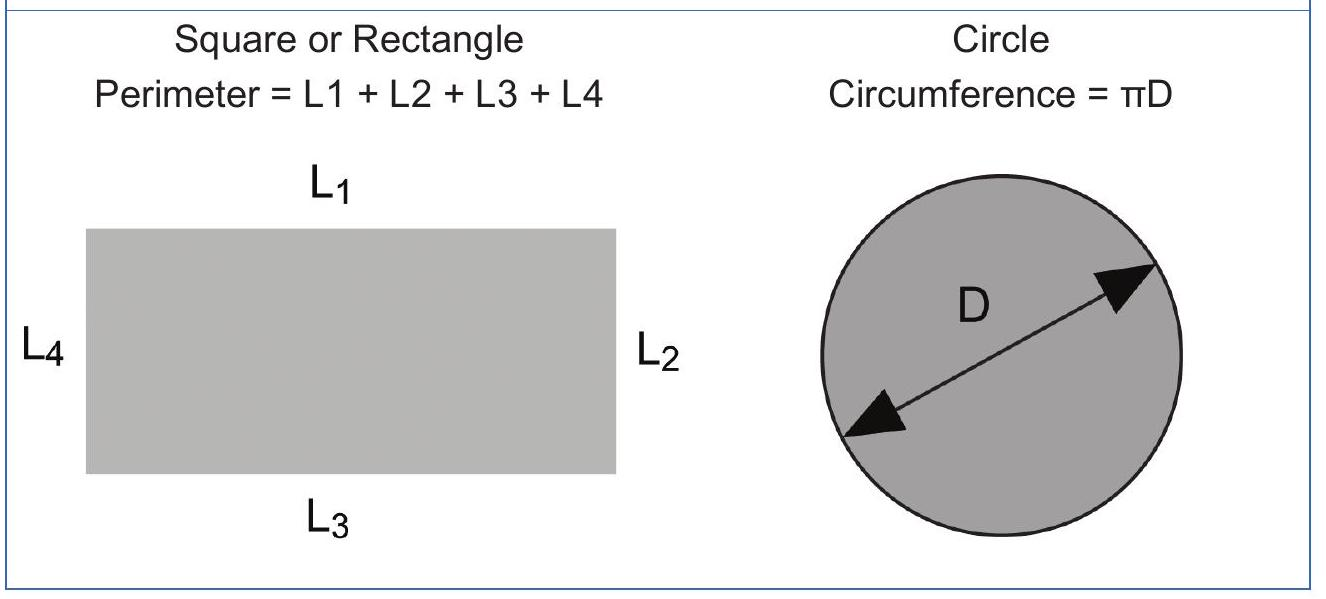
\includegraphics[max width=\textwidth]{2022_09_11_72dbedc910e6e984560cg-25}

Example - Rectangle

Find the perimeter of the following rectangle:

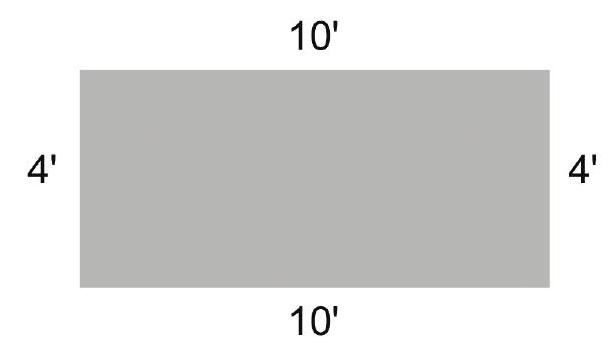
\includegraphics[max width=\textwidth]{2022_09_11_72dbedc910e6e984560cg-25(1)}

$\mathrm{P}=10^{\prime}+4^{\prime}+10^{\prime}+4^{\prime}=28^{\prime}$

\section{Practice Problems - Perimeter and Circumference}
\begin{enumerate}
  \item Find the perimeter or circumference of the following items:\\

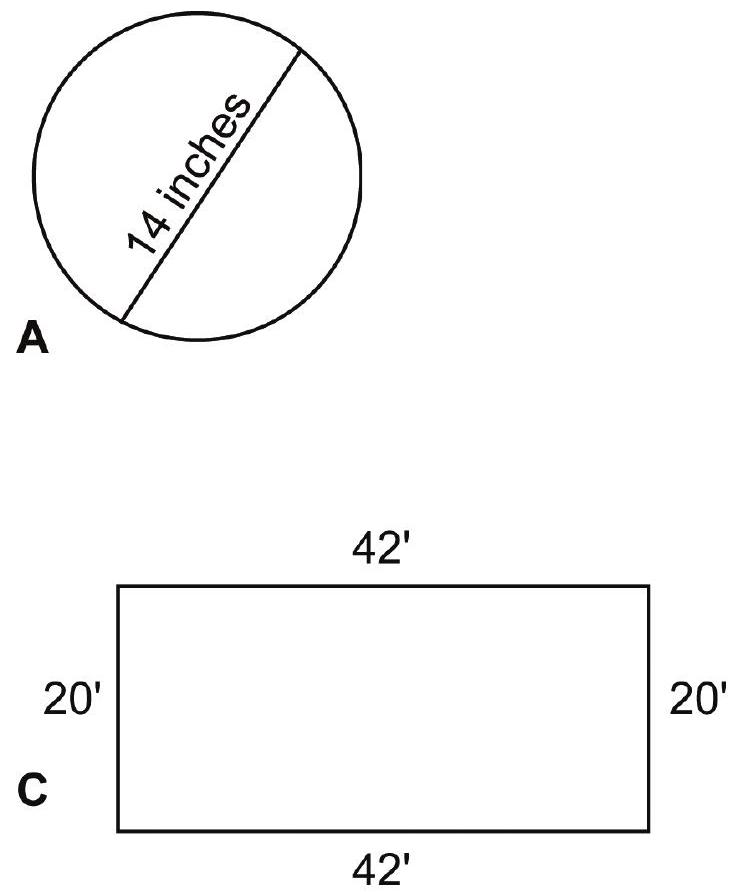
\includegraphics[max width=\textwidth]{2022_09_11_72dbedc910e6e984560cg-26}
\end{enumerate}
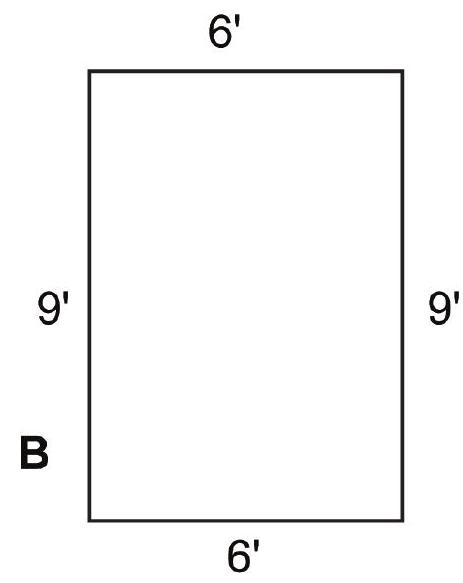
\includegraphics[max width=\textwidth]{2022_09_11_72dbedc910e6e984560cg-26(1)}

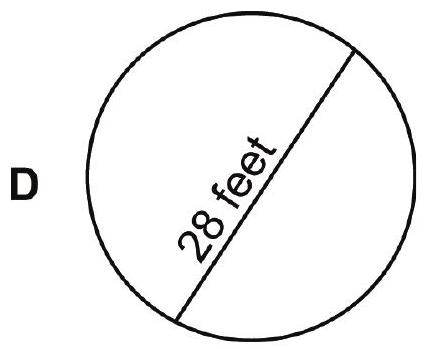
\includegraphics[max width=\textwidth]{2022_09_11_72dbedc910e6e984560cg-26(2)}

D ${ }^{12}$ Cross-sectional Area - The area at right angles to the length of a pipe or basin. ${ }^{13}$ Radius - A line from the center of a circle or sphere to the circumference of the circle or surface of the sphere.

\section{Finding Area}
Units

Area is an expression of the square unit measurement of the surface of an item or a parcel of land. The area on top of a sedimentation basin is called the surface area. The area of the end of a pipe is called the cross-sectional area ${ }^{12}$. Area is usually expressed in squared terms such as square inches $\left(\mathrm{in}^{2}\right)$ or square feet $\left(\mathrm{ft}^{2}\right)$. Land may also be expressed in terms of sections (1 square mile) or acres $\left(43,560 \mathrm{ft}^{2}\right)$ or in the metric system as hectares $\left(10,000 \mathrm{~m}^{2}\right)$.

Formula for a Rectangle

The area of a rectangle is found by multiplying the length times the width.

Where:

$\mathrm{L}=$ length $\quad \mathrm{W}=$ width

Formula for a Circle

The surface area of a circle is determined by multiplying pi times the radius squared $\left(\mathrm{r}^{2}\right)$

Where:

$\mathrm{A}=$ area $\pi=$ Greek letter pi

$r=$ radius $^{13}$ of a circle $\pi=3.1416$

Radius is one-half of the diameter

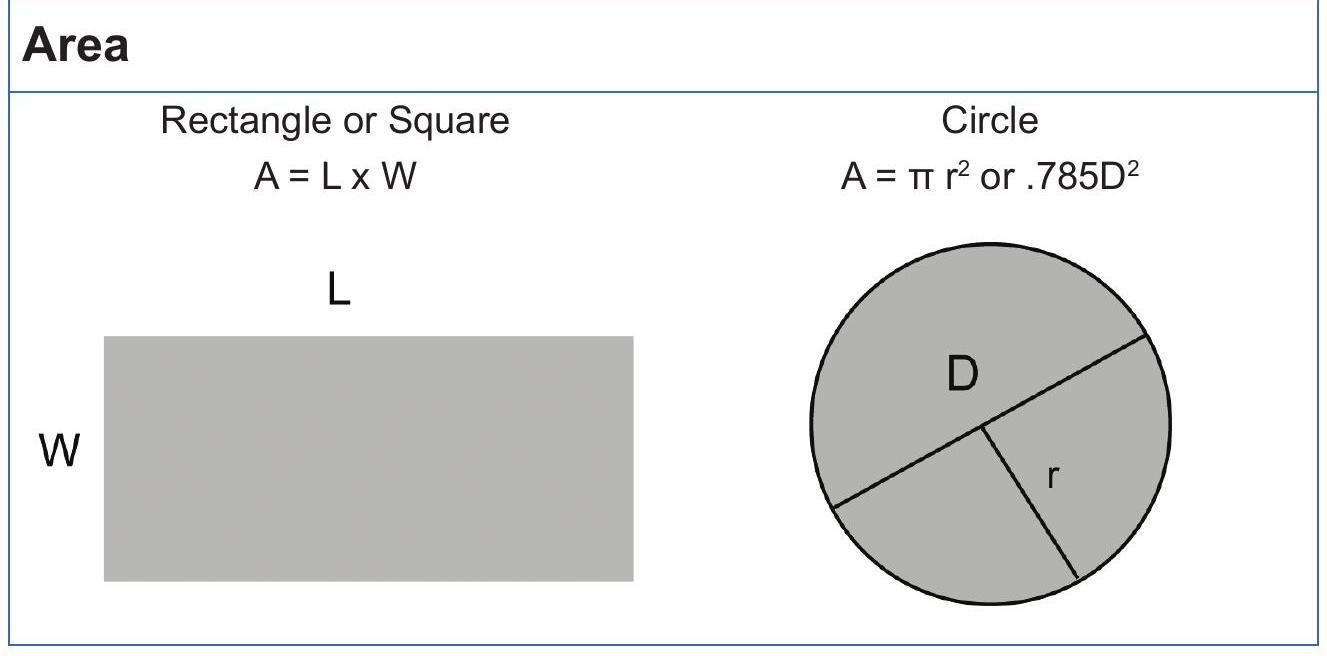
\includegraphics[max width=\textwidth]{2022_09_11_72dbedc910e6e984560cg-27}

Example - Rectangle

Find the area of the following rectangle:

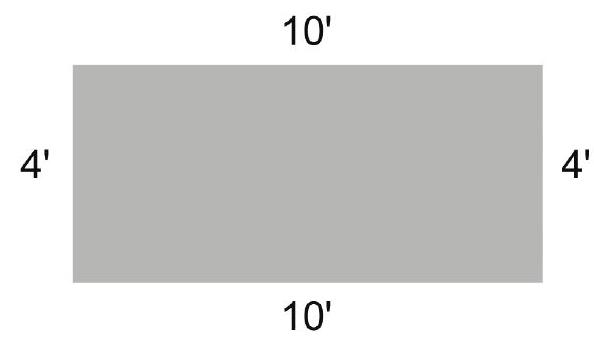
\includegraphics[max width=\textwidth]{2022_09_11_72dbedc910e6e984560cg-27(1)}

$\mathrm{A}=4^{\prime} \times 10^{\prime}=40 \mathrm{ft}^{2}$

This is the same as saying that 40 individual pieces of paper one foot by one foot could be placed on this surface.

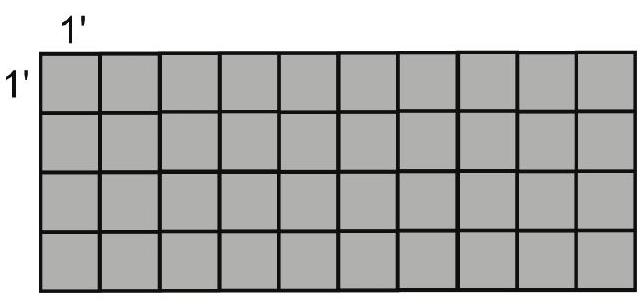
\includegraphics[max width=\textwidth]{2022_09_11_72dbedc910e6e984560cg-27(2)}

Example-Circle

Find the surface area of the following circle with a radius of $5 \mathrm{ft}$ :

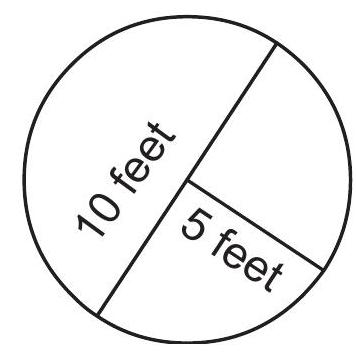
\includegraphics[max width=\textwidth]{2022_09_11_72dbedc910e6e984560cg-27(3)}
$$
\begin{aligned}
& \mathrm{A}=\pi \times \mathrm{r}^{2} \quad \mathrm{~A}=.785 \times \mathrm{D}^{2} \\
& \mathrm{A}=\pi \times 5^{2} \quad \mathrm{Or} \quad \mathrm{A}=.785 \times 10^{2} \\
& \mathrm{A}=\pi \times 25 \mathrm{ft}^{2} \quad \text { Or } \quad \mathrm{A}=.785 \times 10 \times 10 \\
& \mathrm{A}=78.5 \mathrm{ft}^{2} \quad \mathrm{~A}=78.5 \mathrm{ft}^{2} 
\end{aligned}
$$

\section{Practice Problems - Area}
\begin{enumerate}
  \item Find the area of the following items:\\

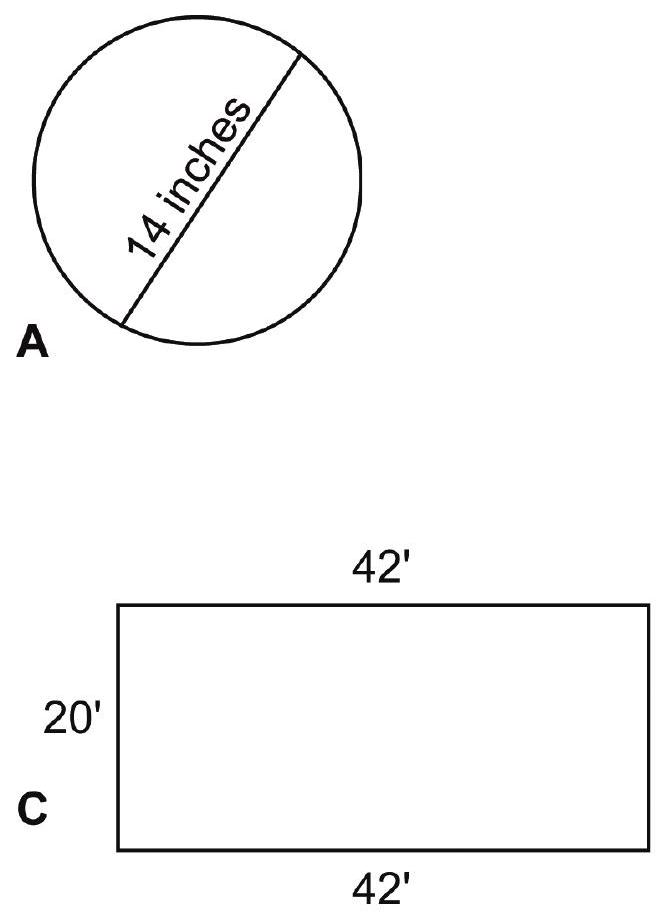
\includegraphics[max width=\textwidth]{2022_09_11_72dbedc910e6e984560cg-28}
\end{enumerate}
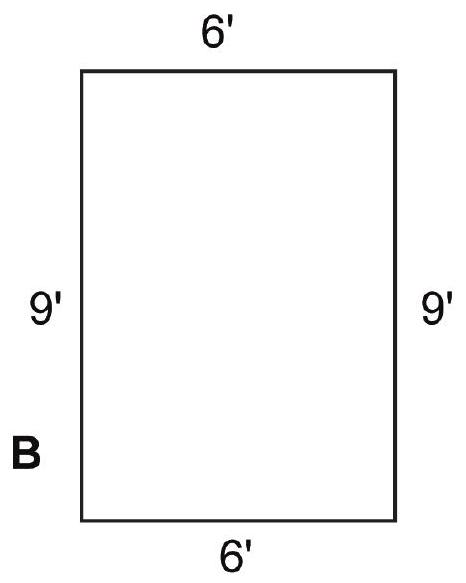
\includegraphics[max width=\textwidth]{2022_09_11_72dbedc910e6e984560cg-28(1)}

20

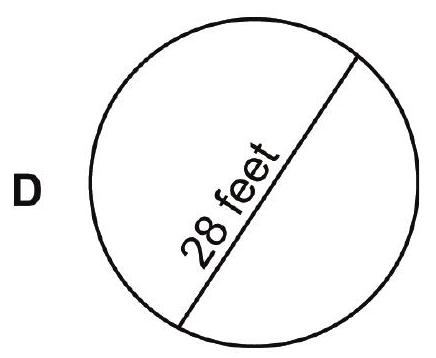
\includegraphics[max width=\textwidth]{2022_09_11_72dbedc910e6e984560cg-28(2)}

\section{Finding the Volume}
Units

Volume ${ }^{14}$ is expressed in cubic units, such as cubic inches $\left(\mathrm{in}^{3}\right)$, cubic feet $\left(\mathrm{ft}^{3}\right)$, acre feet $\left(1\right.$ Acre foot $\left.=43,560 \mathrm{ft}^{3}\right)$, etc.

Formula for Rectangular Object

The volume of a rectangular object is obtained by multiplying the length times the width times the depth or height.
$$
\begin{array}{lll}
\mathrm{V}=\mathrm{L} \times \mathrm{W} \times \mathrm{D} & \text { Where: } \mathrm{L}=\text { length } & \mathrm{W}=\text { width } \\
\mathrm{D}=\text { depth } \quad \text { or } & \mathrm{H}=\text { height }
\end{array}
$$
Formula for a Cylinder

The volume of a cylinder ${ }^{15}$ (such as a piece of pipe or a tank) is equal to its height times pi times the radius of the cylinder squared. The length (L) and height $(\mathrm{H})$ of a cylinder are the same dimension.
$$
\begin{array}{lll}
\mathrm{V}=\mathrm{Hx} \pi \mathrm{r}^{2} & \text { Where: } & \pi=3.1416 \\
\text { or } \mathrm{V}=\mathrm{H} \times .785 \mathrm{D}^{2} & \mathrm{r}=\text { radius of the cylinder } \\
& \mathrm{H}=\text { height or length of the cylinder }
\end{array}
$$
${ }^{14}$ Volume - The amount of space occupied by or contained in an object. Measured by the number of cubes, each with an edge 1 unit long that can be contained in the object. ${ }^{15}$ Cylinder - A solid or hollow figure, traced out when a rectangle rotates using one of its sides as the axis of the rotation.

\section{Volume}
Rectangle or Square

$\mathrm{V}=\mathrm{L} \times \mathrm{W} \times \mathrm{D}$

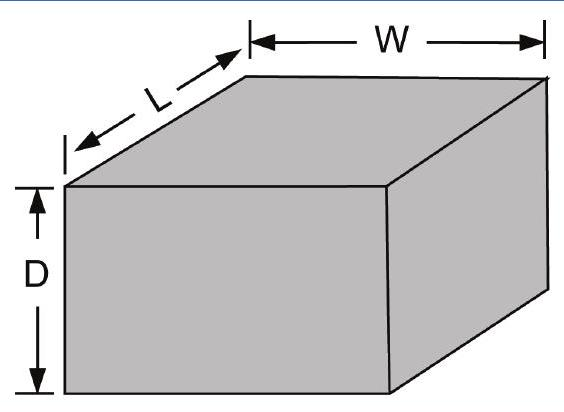
\includegraphics[max width=\textwidth]{2022_09_11_72dbedc910e6e984560cg-29}

Cylinder

$\mathrm{V}=\mathrm{H} \times \pi \mathrm{r}^{2}$ or $\mathrm{V}=\mathrm{H} x .785 \mathrm{D}^{2}$\\

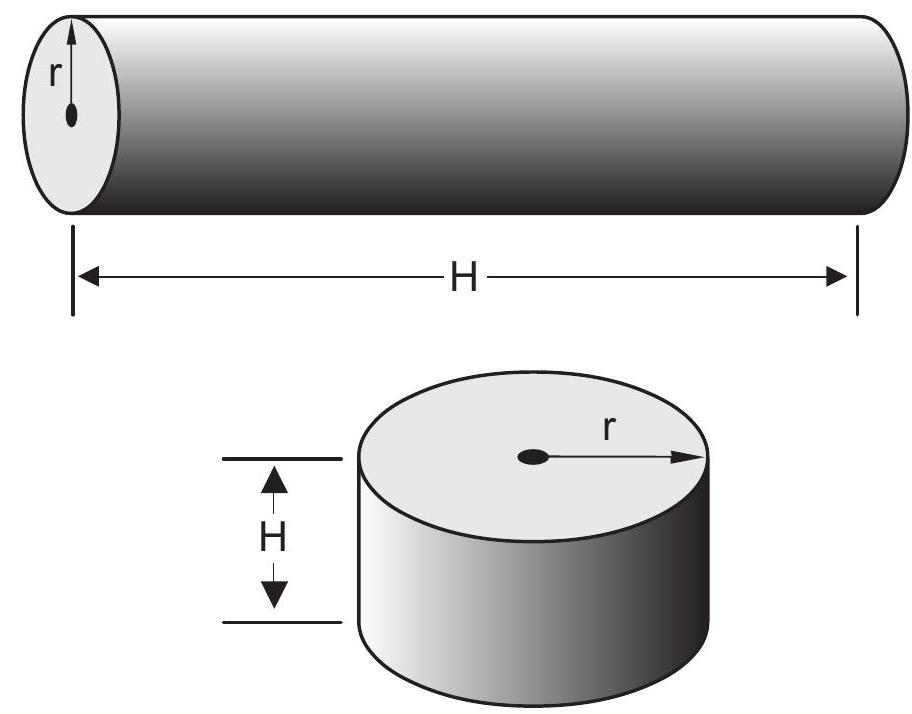
\includegraphics[max width=\textwidth]{2022_09_11_72dbedc910e6e984560cg-29(1)}Example - Volume

Find the volume in cubic feet of the sedimentation basin below:

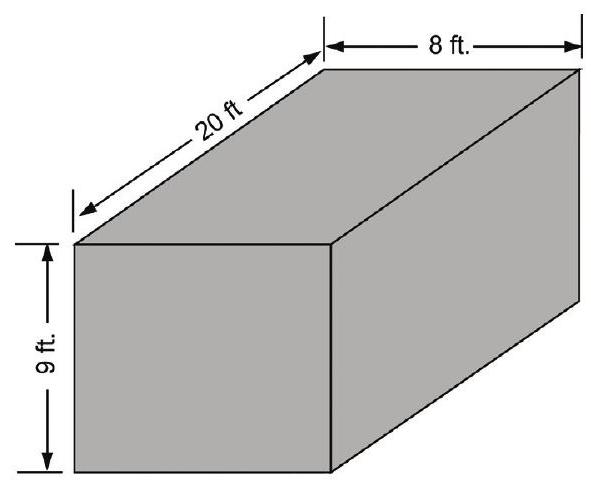
\includegraphics[max width=\textwidth]{2022_09_11_72dbedc910e6e984560cg-30}

$\mathrm{V}=\mathrm{L} \times \mathrm{W} \times \mathrm{D}$

$\mathrm{V}=20 \mathrm{ft} \times 8 \mathrm{ft} \times 9 \mathrm{ft}$

$\mathrm{V}=1,440 \mathrm{ft}^{3}$

Example - Cylinder

Find the volume of a tank 20 feet in diameter and 15 feet tall.

Volume $=\mathrm{Hx} \pi \mathrm{r}^{2}$ or Volume $=\mathrm{H} \mathrm{x} .785 \mathrm{D}^{2}$

The radius of a circle is one-half the diameter. Since the diameter is 20 feet, the radius is 10 feet.

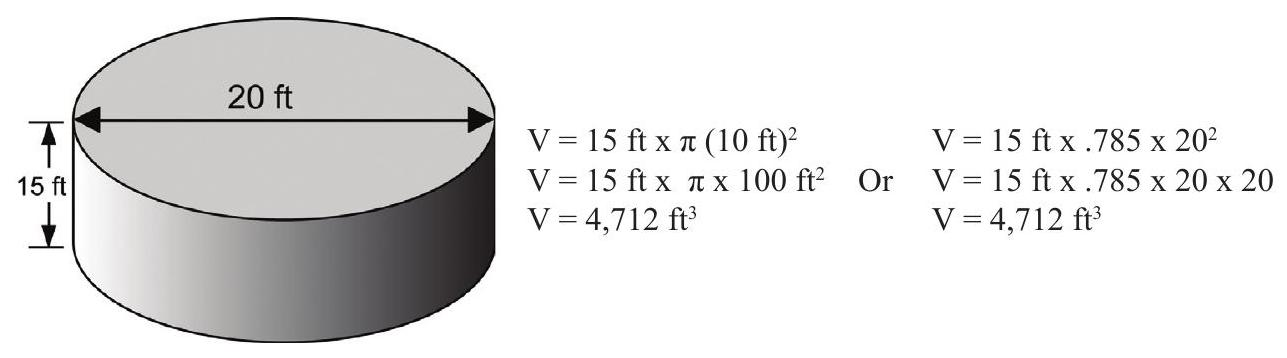
\includegraphics[max width=\textwidth]{2022_09_11_72dbedc910e6e984560cg-30(1)}

\section{Practice Problems - Volume}
\begin{enumerate}
  \item Find the volume of the following:\\
A. A 3-inch pipe 200 feet long. (Hint, change the diameter of the pipe from inches to feet by dividing by 12.)\\
B. A fuel tank 4 feet in diameter and 10 feet long.\\
C. A chlorine barrel that is 20 inches in diameter and 42 inches tall.\\
D. A trench $2.5$ feet wide, 6 feet deep, and 60 feet long.
\end{enumerate}
\section{Working with Percent}
Definition

Percent means parts of 100 parts. The symbol for percent is $\%$. We use percent to describe portions of the whole. For instance, if a tank is $1 / 2$ full, we say that it contains $50 \%$ of the original solution. We also use percent to describe the portion of a budget spent or a project completed. For example, "There is only $25 \%$ of the budgeted amount remaining." "The water line project is $80 \%$ complete."

\section{How Expressed}
Percentage is expressed as a whole number with a \% sign after it, except when it is used in a calculation. In a calculation, percent is expressed as a decimal. The decimal is obtained by dividing the percent by 100 . For instance, $11 \%$ is expressed as the decimal $0.11$, since $11 \%$ is equal to $11 / 100$. This decimal is obtained by dividing 11 by 100 .

\section{Finding Percentage}
To determine what percentage a part is of the whole, divide the part by the whole.

\section{Example $1-$ Percent}
There are 80 water meters to read, Jim has finished 24 of them. What percentage of the meters have been read?

$24 \div 80=0.30$

The $0.30$ is converted to percent by multiplying the answer by 100 .

$0.30 \times 100=30 \%$

Thus $30 \%$ of the 80 meters have been read.

\section{Finding the Whole}
To determine the whole when the part and its percentage is given, divide the part by the percentage.

The part

7 lbs.

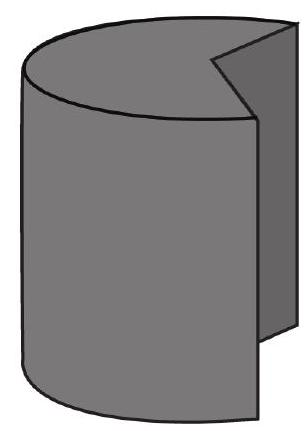
\includegraphics[max width=\textwidth]{2022_09_11_72dbedc910e6e984560cg-31}

The whole $10.8 \mathrm{lbs}$.

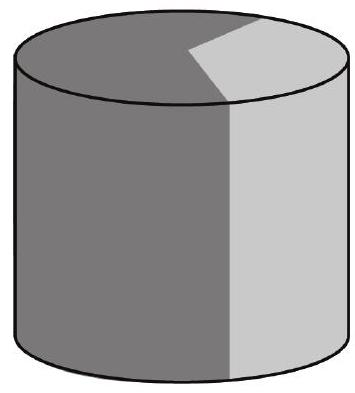
\includegraphics[max width=\textwidth]{2022_09_11_72dbedc910e6e984560cg-31(1)}

\section{Example 2 - Percent}
How much $65 \%$ calcium hypochlorite is required to obtain 7 pounds of pure chlorine? The part is the 7 pounds, which is $65 \%$ of the whole.

\begin{enumerate}
  \item Convert the percentage to a decimal by dividing by 100 .
\end{enumerate}
$65 \% \div 100=0.65$

\begin{enumerate}
  \setcounter{enumi}{2}
  \item Divide the part by the decimal equivalent of the percentage.
\end{enumerate}
$7 \mathrm{lbs} \div 0.65=10.769-$ rounding $10.8 \mathrm{lbs}$.

\section{Changing Decimals to Percent}
To change the percent obtained above to the decimal equivalent, divide the percent by $100 .$

Example - Changing Decimals to Percent

Change $30 \%$ to a decimal.

$30 \% \div 100=0.30(0.30$ is the decimal equivalent of $30 \%$.)

\section{Percentage of a Number}
To find the percentage of a number, multiply the number by the decimal equivalent of the percentage given in the problem.

Example - Percentage

What is $28 \%$ of $286 ?$

\begin{enumerate}
  \item Change the $28 \%$ to a decimal equivalent.
\end{enumerate}
$28 \% \div 100=0.28$

\begin{enumerate}
  \setcounter{enumi}{2}
  \item Multiply $286 \times 0.28=80$
\end{enumerate}
$28 \%$ of 286 is $80.80$ is $28 \%$ of 286 .

Increase a Value by a Percent

To increase a value by a percent, add the decimal equivalent of the percent to " 1 ," and multiply it times the number. Example - Increasing a Value by a Percent

A filter bed will expand $25 \%$ during backwash. If the filter bed is 36 inches deep, how deep will it be during backwash?

\begin{enumerate}
  \item Change the percent to a decimal.
\end{enumerate}
$$
25 \% \div 100=0.25
$$

\begin{enumerate}
  \setcounter{enumi}{2}
  \item Add the whole number 1 to this value.
\end{enumerate}
$$
1+0.25=1.25
$$

\begin{enumerate}
  \setcounter{enumi}{3}
  \item Multiply times the value.
\end{enumerate}
$$
36 \text { in } \times 1.25=45 \text { inches }
$$

\section{Percentage Concentrations}
The concentration of chemicals, such as fluoride and hypochlorites, is commonly expressed as a percentage.

\section{Example - Percentage Concentrations}
A chlorine solution was made to have a $4 \%$ concentration. It is often desirable to determine this concentration in $\mathrm{mg} / \mathrm{L}$. This is relatively simple: the $4 \%$ is four percent of a million.

To find the concentration in $\mathrm{mg} / \mathrm{L}$ when it is expressed in percent, do the following:

\begin{enumerate}
  \item Change the percent to a decimal.
\end{enumerate}
$$
4 \% \div 100=0.04
$$

\begin{enumerate}
  \setcounter{enumi}{2}
  \item Multiply times a million.
\end{enumerate}
$$
0.04 \times 1,000,000=40,000 \mathrm{mg} / \mathrm{L}
$$
We get the million because a liter of water weighs $1,000,000 \mathrm{mg} .1 \mathrm{mg}$ in 1 liter is 1 part in a million parts ( $\mathrm{ppm}) .1 \%=10,000 \mathrm{mg} / \mathrm{L}$.

\section{Practice Problems - Percentage}
A. $25 \%$ of the chlorine in a 30 -gallon vat has been used. How many gallons are remaining in the vat?

B. The annual public works budget is $\$ 147,450$. If $75 \%$ of the budget should be spent by the end of September, how many dollars are to be spent? How many dollars will be remaining?

C. A 75 pound container of calcium hypochlorite has a purity of $67 \%$. What is the total weight of the calcium hypochlorite? D. $3 / 4$ is the same as what percentage?

E. A $2 \%$ chlorine solution is what concentration in $\mathrm{mg} / \mathrm{L}$ ?

F. A water plant produces 84,000 gallons per day. 7,560 gallons are used to backwash the filter. What percentage of water is used to backwash?

G. The average day winter demand ${ }^{16}$ of a community is 14,500 gallons. If the summer demand is estimated to be $72 \%$ greater than the winter, what is the estimated summer demand? ${ }^{16}$ Demand - When related to use, the amount of water used in a period of time. The term is in reference to the "demand" put onto the system to meet the need of customers.

\section{Pump Efficiency}
Horsepower

There are three types of horsepower associated with a pumping installation:

\begin{itemize}
  \item Electrical Horsepower (EHp) - The horsepower that is purchased from the power company.

  \item Brake Horsepower (BHp) - The horsepower that is the output of the electric motor. This is the input horsepower to the pump.

  \item Water Horsepower (WHp) - The horsepower that is the output of the pump.

\end{itemize}
\section{Process - Pump or Motor}
To determine the efficiency of a pump or motor, divide the output horsepower by the input horsepower. Then multiply the result by 100 to change the decimal into percent.

$\frac{\text { Output Horsepower }}{\text { Input Horsepower }} \times 100=\%$ efficiency

Process - When \% is Given

If the efficiency of each unit is known and you wish to determine the efficiency of the entire pump station, then merely multiply the decimal equivalency of the two percentages together.

Efficiency of Motor $x$ Efficiency of Pump $=$ Station $\%$ Example 1 - Pump Efficiency

It has been determined that the water horsepower of a pump is $5 \mathrm{Hp}$ and the brake horsepower output of the motor is $7.2 \mathrm{Hp}$. What is the efficiency of the motor?

$\frac{5 \mathrm{WHp}}{7.2 \mathrm{BHp}} \times 100=69.4 \%$

Example 2 - Pump Efficiency

If a motor is $90 \%$ efficient and the output is $7.5 \mathrm{BHp}$, what is the electrical horsepower requirement?

$\frac{7.5 \mathrm{BHp}}{0.90}=8.3 \mathrm{EHp}$

Example 3 - Well Efficiency

If a pump is $70 \%$ efficient and the motor is $90 \%$ efficient, what is the efficiency of the well?

\begin{enumerate}
  \item Change the efficiency into decimals by dividing each by 100 .
\end{enumerate}
$\frac{70 \%}{100}=0.70, \frac{90 \%}{100}=0.90$

\begin{enumerate}
  \setcounter{enumi}{2}
  \item Multiply the two values.
\end{enumerate}
$0.70 \times 0.90=0.63$

\begin{enumerate}
  \setcounter{enumi}{3}
  \item Multiply the value by 100 to convert the decimal to a percentage.
\end{enumerate}
$0.63 \times 100=63 \%$

\section{Practice Problems - Efficiency}
A. The water horsepower of a pump is $10 \mathrm{Hp}$, and the brake horsepower output of the motor is $15.4 \mathrm{Hp}$. What is the efficiency of the pump?

B. The water horsepower of a pump is $25 \mathrm{Hp}$, and the brake horsepower output of the motor is $48 \mathrm{Hp}$. What is the efficiency of the pump?

C. The efficiency of a well pump is determined to be $75 \%$. The efficiency of the motor is estimated at $94 \%$. What is the efficiency of the well?

D. If a motor is $85 \%$ efficient and the output of the motor is determined to be 10

$\mathrm{BHp}$, what is the electrical horsepower requirement of the motor? E. The water horsepower of a well with a submersible pump has been calculated at 8.2 WHp. The output of the electric motor is measured as $10.3 \mathrm{BHp}$. What is the efficiency of the pump?

\section{Making Conversions}
Use

Conversions are a process of changing the units of a number in order to make the number usable in a specific instance. Common conversions in water works include the following:

\begin{itemize}
  \item gpm to cfs

  \item Million gallons to acre feet

  \item Cubic feet to acre feet

  \item Cubic feet of water to weight

  \item Cubic feet of water to gallons

  \item Gallons of water to weight

  \item gpm to MGD ${ }^{17}$

  \item psi to feet of head ${ }^{18}$

\end{itemize}
\section{Working with Formulas}
To use a formula, you must change the units of the data given to meet the requirements of the formula.

\section{Example - Formulas}
The formula for finding velocity ${ }^{19}$ in a pipe is $\mathrm{V}=\mathrm{Q} \div \mathrm{A}$, where $\mathrm{Q}$ is the flow in cubic feet per second. We most often measure flow in gallons per minute. To use this formula, we must often convert the flow from gpm to cfs.

\section{What Is a Conversion?}
A conversion is a number that is used to multiply or divide into another number in order to change the units of the number.

\section{Known Conversions}
In most instances, the conversion factor cannot be derived. It must be known. Therefore, tables such as the one below are used to find the common conversions.

\section{Committing to Memory}
Most operators memorize some standard conversions. This happens as a result of using the conversions, not as a result of attempting to memorize them. ${ }^{17}$ MGD (Million gallons per day) - A unit of flow and a unit of volume. ${ }^{18} \mathrm{Head}$ - The measure of the pressure of water expressed as height of water in feet: 1 psi $=2.31$ feet of head. ${ }^{19}$ Velocity - The speed at which water moves, expressed in feet per second.

\begin{tabular}{|l|l|}
\hline
Some Common Conversions & Weight \\
\hline
Linear Measurements & $1 \mathrm{ft}^{3}$ of water $=62.4 \mathrm{lbs}$ \\
\hline
1 inch $=2.54 \mathrm{~cm}$ & $1 \mathrm{gal}=8.34 \mathrm{lbs}$ \\
$1 \mathrm{foot}=30.5 \mathrm{~cm}$ & $1 \mathrm{lb}=453.6 \mathrm{grams}$ \\
$1 \mathrm{~meter}=100 \mathrm{~cm}=3.281 \mathrm{feet}=39.4$ inches 1 & $1 \mathrm{~kg}=1000 \mathrm{~g}=2.2 \mathrm{lbs}$ \\
acre $=43,560 \mathrm{ft}^{2}$ & $1 \%=10,000 \mathrm{mg} / \mathrm{L}$ \\
$1 \mathrm{yard}=3 \mathrm{feet}$ & $1 \mathrm{pound}=16 \mathrm{oz} \mathrm{dry} \mathrm{wt}$ \\
 & $1 \mathrm{ft}^{3}=62.4 \mathrm{lbs}$ \\
\hline
Volume & Pressure \\
\hline
$1 \mathrm{gal}=3.78$ liters & $1 \mathrm{ft}$ of head $=0.433 \mathrm{psi}$ \\
$1 \mathrm{ft}=7.48$ gal & $1 \mathrm{psi}=2.31 \mathrm{ft}$ of head \\
$1 \mathrm{~L}=1000 \mathrm{~mL}$ &  \\
$1 \mathrm{gal}=16 \mathrm{cups}$ &  \\
\hline
Flow &  \\
\hline
$1 \mathrm{cfs}=448 \mathrm{gpm}$ &  \\
$1 \mathrm{gpm}=1440 \mathrm{gpd}$ &  \\
\hline
\end{tabular}

\section{Selecting a Conversion}
The key to selecting which conversion to use is to look at the units. If you wish to convert cubic feet of water to pounds, then you need a conversion that has both of these units $\left(1 \mathrm{ft}^{3}\right.$ of water $\left.=62.4 \mathrm{lbs}\right)$.

\section{Complex Process}
The process of converting units can be highly complex and require several steps. A working understanding of the processes used requires a basic understanding of algebra. Because this is outside of the scope of this material, a process that does not require the understanding of algebra is described below. This process works only if there is an existing conversion and only a single conversion is required.

\section{Straight Line Conversion}
The technique described below is for working with straight line conversions. A straight line conversion is one that is direct: gpm to $\mathrm{cfs}$, gal to liters, gallons to pounds, etc.

\section{Process}
The best way to describe this process is with an example. Example - Straight Line Conversion

Convert $865 \mathrm{gpm}$ to cfs.

\begin{enumerate}
  \item Place the known value on the paper with the units as a fraction and with 1 as the denominator to that fraction.

  \item Place a multiplication sign $(\mathrm{x})$ after the units.

  \item Place a straight line after the $x$.

  \item Follow the straight line with an equal sign $(=)$.

\end{enumerate}
$$
865 \frac{\mathrm{gpm}}{1} \mathrm{x}
$$

\begin{enumerate}
  \setcounter{enumi}{5}
  \item Ask the following question, "What units do I want to get rid of?"
\end{enumerate}
$$
865 \frac{\mathrm{gpm}}{1} \times \frac{?}{\mathrm{gpm}}=
$$

\begin{enumerate}
  \setcounter{enumi}{6}
  \item Place this unit under the straight line. In this case, we want to get rid of the gpm.

  \item Ask yourself, "What units do we want when we get done?"

  \item Place this unit above the straight line. The original question ask that we convert gpm to cfs. So cfs is what we want when we get done.

  \item Find a conversion that goes between these two units. From the conversion table, we find the following conversion:

\end{enumerate}
$1 \mathrm{cfs}=448 \mathrm{gpm}$

\begin{enumerate}
  \setcounter{enumi}{10}
  \item Place the conversion next to the proper units above or below the line. In our example, the conversion was 448 gpm, so the 448 goes below the line next to its proper units.
\end{enumerate}
$$
865 \frac{\mathrm{gpm}}{1} \times \frac{1 \mathrm{cfs}}{448 \mathrm{gpm}}=
$$

\begin{enumerate}
  \setcounter{enumi}{11}
  \item Solve the problem. The information above could be rewritten into a fraction.
\end{enumerate}
$$
\mathrm{cfs}=\frac{865 \mathrm{gpm} \times 1 \mathrm{cfs}}{1 \times 448 \mathrm{gpm}}=\frac{865 \mathrm{gpm} \times 1 \mathrm{cfs}}{448 \mathrm{gpm}}=1.92 \mathrm{cfs}
$$

\section{Practice Problems - Conversion}
\begin{enumerate}
  \item Convert the following:\\
A. $750 \mathrm{ft}^{3}$ of water to gallons\\
B. 50 gallons of water to pounds\\
C. $560 \mathrm{gpm}$ to $\mathrm{cfs}$\\
D. 4 lbs to ounces E. $128 \mathrm{ft}^{3}$ of water to weight in pounds
\end{enumerate}
F. 340 in $^{2}$ to $\mathrm{ft}^{2}$

G. $3.4 \mathrm{cfs}$ to $\mathrm{gpm}$

H. $\quad$ H. $65 \mathrm{ft}^{3}$ to $\mathrm{yd}^{3}$

I. 3,000 gallons to $\mathrm{ft}^{3}$

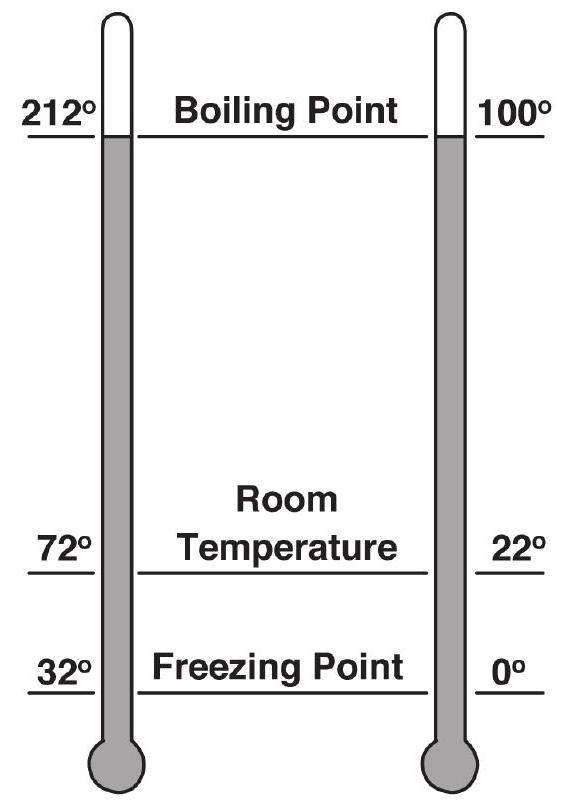
\includegraphics[max width=\textwidth]{2022_09_11_72dbedc910e6e984560cg-39}

Fahrenheit Celsius

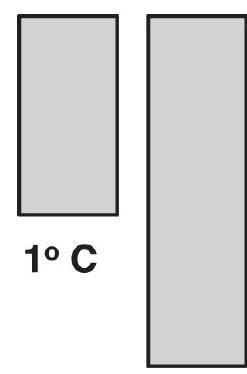
\includegraphics[max width=\textwidth]{2022_09_11_72dbedc910e6e984560cg-39(1)}

$1^{0} \mathrm{~F}$

N. 2.4 MGD to gpm

O. 65 pints to gallons

P. $2.5 \mathrm{ft}^{2}$ to square inches

Q. 7 yards to feet

R. 36,000 gpd to gpm

S. $125 \mathrm{gpm}$ to $\mathrm{gph}$

\section{Temperature Conversion}
\section{Two Scales}
There are two scales used to report temperature: the English scale of Fahrenheit and the metric scale of Celsius. There are two classic equations used to convert between these two scales:

${ }^{\circ} \mathrm{C}=5 / 9\left({ }^{\circ} \mathrm{F}-32^{\circ}\right)$

${ }^{\circ} \mathrm{F}=\left(9 / 5 \mathrm{X}^{\circ} \mathrm{C}\right)+32^{\circ}$

\section{Confusion}
Typically, these two formulas provide more confusion than clarity. The following is our attempt to share a method that we find helpful in making these conversions.

\section{The Scales}
To understand how to make these conversions, start with comparing the two scales. With the Fahrenheit scale, water freezes at $32^{\circ}$ and boils at $212^{\circ}$. On the Celsius scale, water freezes at $0^{\circ}$ and boils at $100^{\circ}$.

\section{Difference of $32^{\circ}$}
We can see that if we want to go from Fahrenheit to Celsius we must start by subtracting $32^{\circ}$. To go from Celsius to Fahrenheit, we must add $32^{\circ}$.

\section{Size of the Division}
The difference between $32^{\circ}$ and $212^{\circ}$ is $180^{\circ}$. This is the difference between water freezing and boiling on the Fahrenheit scale. The difference between freezing and boiling on the Celsius scale is $100^{\circ}$. Therefore, we can see that each $1^{\circ}$ change in the Celsius scale is the same as a $1.8^{\circ}$ change in the Fahrenheit scale.

\section{Changing Scales}
As a result, to change from Celsius to Fahrenheit, we must multiply the result by $1.8$. To change from Fahrenheit to Celsius we must divide by $1.8$.

\section{Final Confusion}
The most confusing part is to determine if you should adjust for the $32^{\circ}$ first or adjust for the size of the scale first. Here are the rules:

Rule 1 - To change ${ }^{\circ} \mathrm{F}$ to ${ }^{\circ} \mathrm{C}$ - subtract $32^{\circ}$ then divide by $1.8$.

Rule 2 - To change ${ }^{\circ} \mathrm{C}$ to ${ }^{\circ} \mathrm{F}$ - multiply by $1.8$ and add $32^{\circ}$.

\section{Conclusion}
We now have two new formulas:
$$
\begin{aligned}
&{ }^{\circ} \mathrm{C}=\frac{{ }^{\circ} \mathrm{F}-32^{\circ}}{1.8} \\
&{ }^{\circ} \mathrm{F}={ }^{\circ} \mathrm{C} X 1.8+32^{\circ}
\end{aligned}
$$
A Third Choice

Several textbooks show a third method of making this conversion. This is a three-step method:

Step $1-\operatorname{Add} 40^{\circ}$ to the existing value.

Step 2 - Multiply by $1.8$ if going to ${ }^{\circ} \mathrm{F}$ and divide by $1.8$ if going to ${ }^{\circ} \mathrm{C}$.

Step 3 - Subtract $40^{\circ}$.

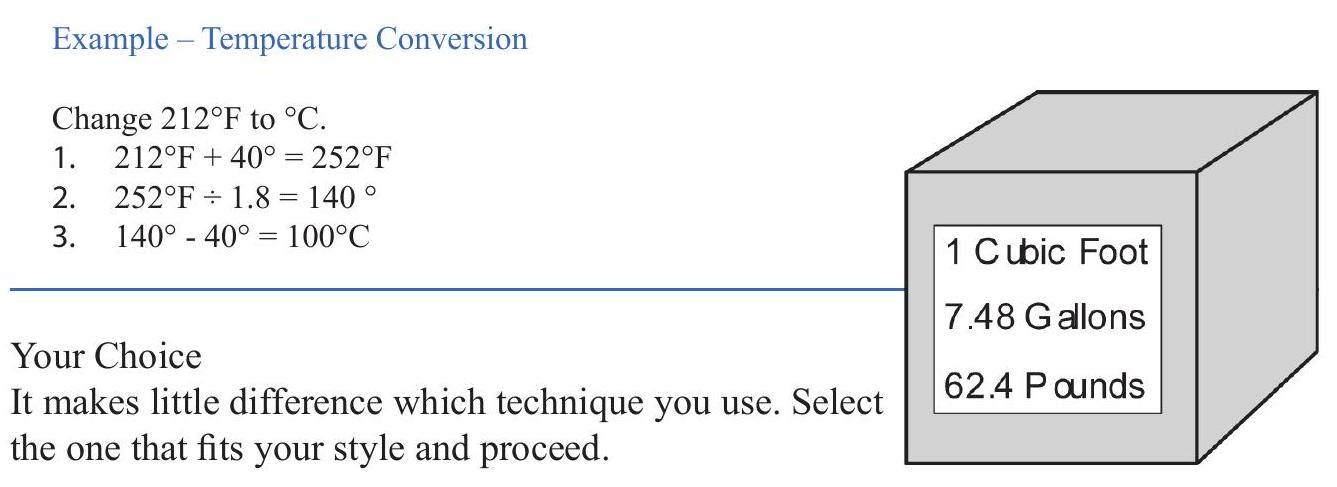
\includegraphics[max width=\textwidth]{2022_09_11_72dbedc910e6e984560cg-41}

\section{Practice Problems - Temperature Conversion}
A. Change $70^{\circ} \mathrm{F}$ to ${ }^{\circ} \mathrm{C}$\\
B. Change $140^{\circ} \mathrm{F}$ to ${ }^{\circ} \mathrm{C}$\\
C. Change $20^{\circ} \mathrm{C}$ to ${ }^{\circ} \mathrm{F}$\\
D. Change $85^{\circ} \mathrm{C}$ to ${ }^{\circ} \mathrm{F}$\\
E. Change $4{ }^{\circ} \mathrm{C}$ to ${ }^{\circ} \mathrm{F}$

\section{Calculating Pressure and Head}
\section{Definition}
Pressure is the weight per unit area. Typical pressure units are pounds per square inch

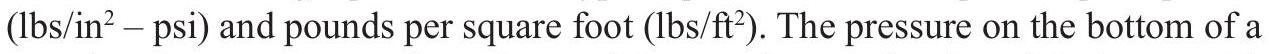
\includegraphics[max width=\textwidth]{2022_09_11_72dbedc910e6e984560cg-41(1)}\\
container is not related to the volume of the container or the size of the bottom. The pressure depends on the height of the fluid in the container. (For more information, see the Hydraulics section of Chapter 2.)

\section{Pressure and Head}
The height of the fluid in a container is referred to as head. Head is a direct measurement in feet and is directly related to pressure.

\section{Relationship Between Feet and Head}
Weight of Water

Water weighs $62.4$ pounds per cubic foot.

The surface of any one side of the cube contains 144 square inches $\left(12\right.$ " x $12^{\prime \prime}=144$ in $^{2}$ ). Therefore, the cube contains 144 columns of water one foot tall and one inch square.

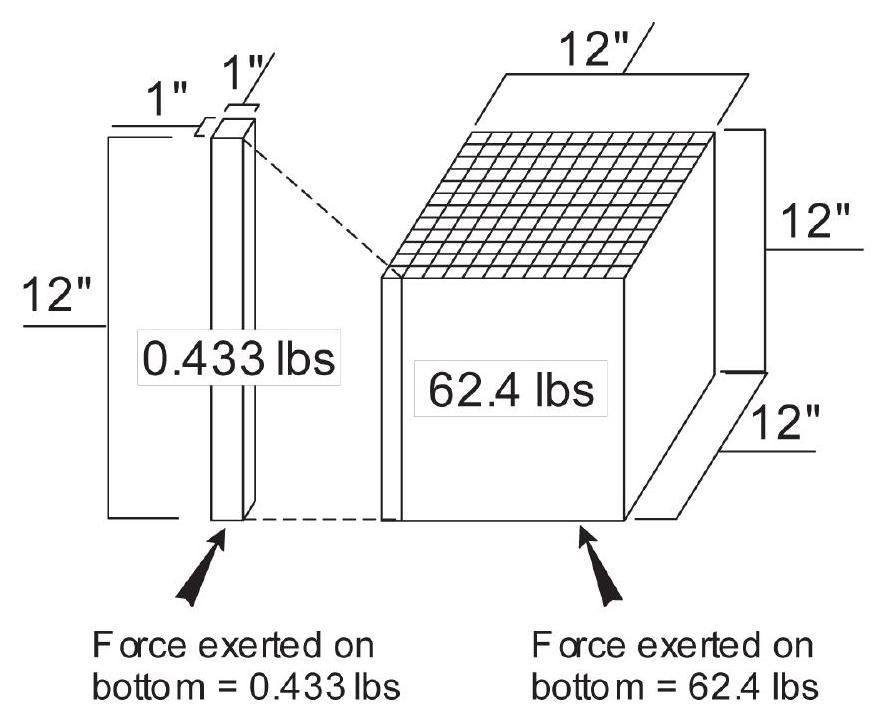
\includegraphics[max width=\textwidth]{2022_09_11_72dbedc910e6e984560cg-42}

The weight of each of these pieces can be determined by dividing the weight of the water in the cube by the number of square inches.

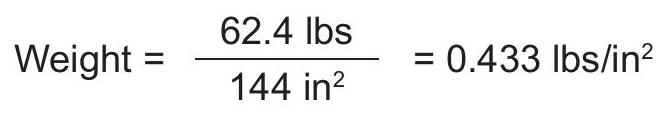
\includegraphics[max width=\textwidth]{2022_09_11_72dbedc910e6e984560cg-42(1)}

or $0.433 \mathrm{psi}$

Since this is the weight of one column of water one foot tall, the true expression would be $0.433$ pounds per square inch per foot of head or $0.433 \mathrm{psi} / \mathrm{ft}$.

What formula do you want here?

Conversion

We now have a conversion between feet of head and psi.

1 foot of head $=0.433 \mathrm{psi}$

While it can be calculated from the relationship above, it is also desirable to know the relationship between pressure and feet of head. In other words, 1 psi represents how many feet of head. This is determined by dividing 1 by $0.433 \mathrm{psi}$.

foot of head $=\frac{1 \mathrm{ft}}{0.433 \mathrm{psi}}=2.31 \mathrm{ft} / \mathrm{psi}$

In other words, if a pressure gauge were reading 10 psi, we know that the height of the water necessary to represent this pressure would be $10 \mathrm{psi} \times 2.31 \mathrm{ft} / \mathrm{psi}=23.1 \mathrm{ft}$. Both Conversions

$1 \mathrm{ft}=0.433 \mathrm{psi}$

$1 \mathrm{psi}=2.31$ feet

Which Conversion to Use

Many operators find having two conversions for the same thing is confusing. They agree that it is best to memorize one and stay with it. The most accurate conversion is the $1 \mathrm{ft}=0.433 \mathrm{psi}$. This is the conversion used in this text.

\section{Example - Conversion}
To convert $40 \mathrm{psi}$ to feet of head, use the standard conversion technique described earlier.
$$
40 \frac{\mathrm{psi}}{1} \times \frac{\mathrm{ft}}{0.433 \mathrm{psi}}=92.4 \text { feet }
$$
Convert 40 feet to psi.
$$
40 \frac{\mathrm{ft}}{1} \mathrm{x} \frac{0.433 \mathrm{psi}}{1 \mathrm{ft}}=17.3 \mathrm{psi}
$$

\section{Another Way}
As you can see, if you are attempting to convert psi to feet, you divide by $0.433$, and if you are attempting to convert feet to psi, you multiply by $0.433$. It can become confusing about when to divide and when to multiply. The above process can be most helpful in making that determination. However, there is another way. Notice that the relationship between psi and feet is almost two to one. It takes slightly more than two feet to make one psi. Therefore, when looking at a problem where the data is in pressure and you want it in feet, we can see that the answer will be at least twice as large as the number we are starting with. For example, if the pressure were $20 \mathrm{psi}$, we know that the head is over 40 feet. Therefore, we must divide by $0.433$ to obtain the correct answer.

\section{Practice Problems - Pressure and Head}
\begin{enumerate}
  \item Make the following conversions:\\
A. Convert a pressure of 45 psi to feet of head.
\end{enumerate}
B. Convert $12 \mathrm{psi}$ to feet of head.

C. Convert 85 psi to feet of head.

D. It is 112 feet in elevation between the top of the reservoir and the watering point. What will the static pressure be at the watering point?

E. A reservoir is 20 feet deep. What will the pressure be at the bottom of the reservoir?

\section{Determining Flow}
Units

Flow is expressed in the English system of measurements using many terms. The most common flow terms include the following:

\begin{itemize}
  \item gpm-Gallons per minute

  \item cfs - Cubic feet per second

  \item gpd-Gallons per day

  \item MGD - Million gallons per day

\end{itemize}
\section{Conversions}
Flow rates can be converted to different units using the conversion process describe above. The most common flow conversions are $1 \mathrm{cfs}=448 \mathrm{gpm}$ and $1 \mathrm{gpm}=1440$ gpd.

Gallons per Day (gpd) to MGD

To convert gallons per day to MGD, divide the gpd by $1,000,000$.

Example - Conversion of gdp to MGD

Convert 125,000 gallons to MGD.

$\frac{125,000 \mathrm{gpd}}{1,000,000}=0.125 \mathrm{MGD}$

Convert 2,300,000 gpd to MGD.

$\frac{2,300,000 \mathrm{gpd}}{1,000,000}=0.2 .3 \mathrm{MGD}$

Conversion of MGD to gpm

There are many instances where the design or plant information is given in MGD, and we wish to have the flow in gpm. This conversion is accomplished in two steps:

\begin{enumerate}
  \item Convert to gpd by multiplying by $1,000,000$.

  \item Convert to gpm by dividing by the number of minutes in a day $(1440 \mathrm{~min} /$ day). Example - Conversion of MGD to gpm

\end{enumerate}
Convert $0.125$ MGD to gpm.

\begin{enumerate}
  \item Convert the flow in MGD to gpd.
\end{enumerate}
$0.125$ MGD x 1,000,000 = 125,000 gpd

\begin{enumerate}
  \setcounter{enumi}{2}
  \item Convert to gpm by dividing by the number of minutes in a day (24 hrs per day $x 60 \mathrm{~min}$ per hour) $1440 \mathrm{~min} /$ day.
\end{enumerate}
$$
\frac{125,000 \mathrm{gpd}}{1,440 \mathrm{~min} / \text { day }}=86.6 \text { or } 87 \mathrm{gpm}
$$
Convert gpd to gpm

The process of converting gpd to gpm is shown in the example above. The process is to divide the flow in gpd by the number of minutes in a day (1440 min/day).

\section{Conversion of gpm to $\mathrm{cfs}$}
The conversion from gpm to cfs is shown in the examples in the above section on conversions. The conversion is $1 \mathrm{cfs}=448 \mathrm{gpm}$.

\section{Determining Flow Equation}
Flow in a pipeline, channel, or stream is found using the equation:

$\mathrm{Q}=\mathrm{V} \times \mathrm{A}$

Where

$Q=$ cubic feet per second (cfs)

$V=$ velocity in feet per second $(\mathrm{ft} / \mathrm{sec})$

$A=$ area in square feet $\left(\mathrm{ft}^{2}\right)$

\section{Example - Determining Flow}
Find the flow in cfs in a 6 -inch line, if the velocity is 2 feet per second.

\begin{enumerate}
  \item Determine the cross-sectional area of the line in square feet. Start by converting the diameter of the pipe to inches.
\end{enumerate}
The diameter is 6 inches: therefore, the radius is 3 inches. 3 inches is $3 / 12$ of a foot or $0.25$ feet.

\begin{enumerate}
  \setcounter{enumi}{2}
  \item Now find the area in square feet.
\end{enumerate}
$$
\begin{aligned}
&A=\pi \times r^{2} \\
&A=\pi \times\left(0.25 \mathrm{ft}^{2}\right. \\
&A=\pi \times 0.0625 \mathrm{ft}^{2} \\
&A=0.196 \mathrm{ft}^{2}
\end{aligned}
$$
Or
$$
\begin{aligned}
&A=0.785 \times D^{2} \\
&A=0.785 \times 0.5^{2} \\
&A=0.785 \times .05 \times .05 \\
&A=0.196 \mathrm{ft}^{2}
\end{aligned}
$$

\begin{enumerate}
  \setcounter{enumi}{3}
  \item Now find the flow.
\end{enumerate}
$\mathrm{Q}=\mathrm{V} \times \mathrm{A}$

$\mathrm{Q}=2 \mathrm{ft} / \mathrm{sec} \times 0.196 \mathrm{ft}^{2}$

$\mathrm{Q}=0.3927 \mathrm{cfs}$ or $0.4 \mathrm{cfs}$

\section{Practice Problems - Flow}
A. Find the flow in MGD when the flow is $34,000 \mathrm{gpd}$.

B. Find the flow in gpm when the total flow for the day is 65,000 gpd.

C. Find the flow in gpm when the flow is $1.3 \mathrm{cfs}$.

D. Find the flow in gpm when the flow is $0.25 \mathrm{cfs}$.

E. Find the flow in a 4-inch pipe when the velocity is $1.5$ feet per second.

\section{Calculating Detention Time}
Detention time is the amount of time that a fluid stays in a container.

Units

Detention time is expressed in units of time. The most common are seconds, minutes, hours, and days.

\section{Calculations}
The simplest way to calculate the detention time is to divide the volume of the container by the flow rate into the container. The theoretical detention time of a container is the same as the amount of time it would take to fill the container if it were empty.

\section{Volume Units}
The most common volume units used are gallons. However, on occasion cubic feet may also be used.

\section{Time Units}
The time units will be in whatever units are used to express the flow. For instance, if the flow is in gpm, then the detention time will be in minutes. If the flow is in gpd, then the detention time will be in days. If in the final result the detention time is in the wrong time units, then simply convert to the appropriate units.

\section{Example - Detention Time}
The reservoir for the village is 85,000 gallons. The well will produce $55 \mathrm{gpm}$. What is the detention time in the tank in hours?
$$
\mathrm{DT}=\frac{85,000 \mathrm{gal}}{55 \mathrm{gpm}}=1,545 \mathrm{~min} \text { or } \frac{1,545 \mathrm{~min}}{60 \mathrm{~min} / \mathrm{hr}}=25.8 \mathrm{hrs}
$$

\section{Practice Problems - Detention Time}
A. How long will it take to fill a 50-gallon hypochlorite tank if the flow is 5 gpm?

B. Find the detention time in a 45,000 gallon reservoir if the flow rate is $85 \mathrm{gpm}$.

C. If the fuel consumption to the boiler is 35 gallons per day, how many days will the 500 gallon tank last?

D. The sedimentation basin of a water plant contains 5,775 gallons. What is the detention time if the flow is $175 \mathrm{gpm}$ ?

\section{Ratio and Proportion}
What is a Ratio?

A ratio is a relationship between two numbers. A ratio can be written using a colon $(1: 2,5: 9,20: 60)$ or a fraction $(1 / 2,5 / 9$, or $20 / 60)$.

What Is a Proportion?

A proportion exists when the relationship between one ratio is the same as the relationship between a second ratio.

How Is This Determined?

To determine if two ratios are proportional, the two are cross-multiplied. If the answers are equal, then they are proportional.

Example 1 - Ratio and Proportion

Determine if $3 / 9$ is proportional to $6 / 18$.

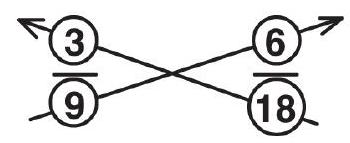
\includegraphics[max width=\textwidth]{2022_09_11_72dbedc910e6e984560cg-47}

$9 \times 6=54$ and $3 \times 18=54$; therefore, the two ratios are proportional.

Example 2 - Ratio and Proportion

Determine if $5 / 9$ and $6 / 20$ are proportional.

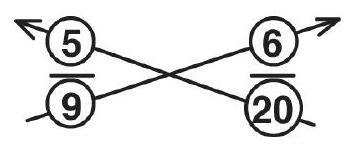
\includegraphics[max width=\textwidth]{2022_09_11_72dbedc910e6e984560cg-47(1)}

$9 \times 6=54$ and $5 \times 20=100$; therefore, the two are not proportional.

\section{So Now What?}
This process is an introduction into the practical use of ratios and proportions used to solve common problems. To use this process, we need to discuss one more major step and then provide some basic rules. The first step is what to do when one part of a ratio is unknown.

\section{The Unknown}
To solve for an unknown portion of a ratio, follow these steps:

Step 1 - Set up the ratios in a proportion format. Place an " $\mathrm{W}$ " in the ratio for the unknown value. Notice that we have set the two ratios up as a proportion with the colon (:) between them.
$$
\frac{2}{15}: \frac{X}{50}
$$
Step 2 - Cross-multiply keeping all numbers as numerators. (We are multiplying both sides of the equestion by the denominators over 1.)

$(15)(\mathrm{X})=(2)(50)$

Step 3 - To get the $\mathrm{X}$ on the left side of the equation, divide both sides by 15 .
$$
\mathrm{X}=\frac{(2)(50)}{15}
$$
Step 4 - Solve for X.
$$
\mathrm{X}=6.67
$$

\section{Practical Application}
Proportion problems deal with larger and smaller values of the same units. For instance, a common proportion problem might be the following:

If it takes 5 pounds of calcium hypochlorite to give the correct dosage in a 35 gallon tank, then how many pounds will it take to make 12 gallons?

Rule 1 - Set up the proportion with the same types of units on one side of the colon. Using our example above, pounds would go on one side and gallons on the other.

Rule 2 - The numerators must contain the same size of units (either larger or small units), and the denominator must contain the same size units (either larger or smaller). For instance:

$\frac{\text { Smaller Value }}{\text { Larger Value }}: \frac{\text { Smaller Value }}{\text { Larger Value }}$

or

$\frac{\text { Larger Value }}{\text { Smaller Value }}: \frac{\text { Larger Value }}{\text { Smaller Value }}$

Rule 3 - Place an " $\mathrm{X}$ " in the unknown value, and solve for " $\mathrm{X}$."

Hint

Using our example above, you can set up a verbal relationship. For instance, 5 pounds is to 35 gallons as $\mathrm{X}$ pounds is to 12 gallons. To place these in the equation, start in the upper left with the 5 pounds. The "is to" represents the equal sign. For instance:

$\frac{5 \mathrm{lbs}}{\mathrm{X}}: \frac{35 \mathrm{gal}}{12 \mathrm{gal}}$

(X) $(35 \mathrm{gal})=(5 \mathrm{lbs})(12 \mathrm{gal})$

$\mathrm{X}=\frac{(5 \mathrm{lbs})(12 \mathrm{gal})}{35 \mathrm{gal}}=1.7 \mathrm{lbs}$

Example 3 - Ratio and Proportion

If one chlorine cylinder is used in 20 days, how many will be used in 100 days?

Step 1 - Set up the proportion.

1 cylinder is to 20 days as $\mathrm{X}$ cylinders is to 100 days.

$\frac{1 \text { cylinder }}{\mathrm{X}}: \frac{20 \text { days }}{100 \text { days }}$

Step 2 - Cross-multiply.

( $\mathrm{X}$ cylinders) $(20$ days $)=(1$ cylinder $)(100$ days $)$

Step 3 - Rearrange the equation to get " $X$ " on the left by its self; divide both sides by 20 days.

$X$ cylinders $=\frac{(1 \text { cylinder })(100 \text { days })}{20 \text { days }}$

Step 4 - Solve for $\mathrm{X}$ cylinders.

$\mathrm{X}=5$ cylinders

\section{Practice Problems - Ratio and Proportion}
A. It takes 6 gallons of chlorine solution to obtain a proper residual when the flow is 45,000 gpd. How many gallons will it take when the flow is 62,000 gpd?

B. A motor is rated at 41 amps average draw per leg at $30 \mathrm{Hp}$. What is the actual $\mathrm{Hp}$ when the draw is 36 amps? C. If it takes 2 operators $4.5$ days to clean an aeration basin, how long will it take three operators to do the same job?

D. If it takes 20 minutes to pump a wet well down with one pump pumping at 125 gpm, then how long will it take if a 200 gpm pump is used?

E. It takes 3 hours to clean 400 feet of collection system using a sewer ball. How long will it take to clean 250 feet?

F. It takes 14 cups of $\mathrm{HTH}$ to make a $12 \%$ solution, and each cup holds 300 grams. How many cups will it take to make a $5 \%$ solution?

\section{Pounds Formula}
Use

One of the most common formulas used by water and wastewater operators is the pounds formula. This formula is used to determine the loading on the plant and its various process units; the loading on the receiving water; and the amount of chemicals needed for a specific function, such as disinfection. The formula can also be used to determine the amount of mixed liquor in the aeration basin and the amount of sludge to be disposed of in the landfill.

\section{Basic Assumption}
The formula assumes that all of the material found in water (TSS, BOD, MLSS, Chlorine, etc.) weighs the same as water, that is, $8.34$ pounds per gallon.

\section{The Formula}
The basic pounds formula is

Lbs = Flow, MG $\times 8.34 \times$ Conc, $\mathrm{mg} / \mathrm{L}$

Where

Lbs $=$ pounds

$M G=$ Flow or volume in millions of gallons

Conc $=$ concentration or dosage in $\mathrm{mg} / \mathrm{L}$

\section{Process}
The process of using the pounds formula to determine pounds of a substance in water is relatively simple. Just plug the values into the appropriate slots and multiply.

However, there are two items that can cause some confusion: flows of less than one million gallons and concentrations in ppm. Flow

Flow and volume are often expressed in gallons per day, gallons per minute and millions of gallons per day. Regardless of how they are expressed, they must be converted to MG in order for them to be placed in this formula. When the flow is in gallons or million gallons per day (MGD), the pounds must be expressed in $1 \mathrm{bs} /$ day.

Flow or Volume in gpd

When a flow or volume is expressed in gallons, it must be converted to MGD by dividing it by $1,000,000$. For instance, a flow of 120,000 gpd is $0.12 \mathrm{MGD}$, and a flow of $40,000 \mathrm{gpd}$ is $0.04 \mathrm{MGD}$.

Flow or Volume in gpm

When a flow or volume is expressed in gpm, it must be first converted to gpd by multiplying by the number of minutes per day (1440) and then divided by $1,000,000$ to get MGD.

Example 1 - Flow

The flow is $250 \mathrm{gpm}$. What is the flow in MGD?

$250 \mathrm{gpm} \times 1440 \mathrm{~min} / \mathrm{day}=360,000 \mathrm{gpd}$

$360,000 \mathrm{gpd} \div 1,000,000=0.36 \mathrm{MGD}$

\section{PPM}
PPM or ppm is an abbreviation for parts per million. Parts per million is the same as $\mathrm{mg} / \mathrm{L}$ (milligrams per liter). While they mean the same, $\mathrm{mg} / \mathrm{L}$ is the preferred and more accepted unit.

\section{Example 2 -Flow}
A water treatment plant feeds alum at a dosage of $26 \mathrm{mg} / \mathrm{L}$. The flow is $2.5 \mathrm{MGD}$. How many pounds of alum are used each day?

$\mathrm{lbs} / \mathrm{day}=\mathrm{MGD} \times 8.34, \mathrm{lbs} / \mathrm{gal} \times \mathrm{Conc}, \mathrm{mg} / \mathrm{L}$

$\mathrm{lbs} / \mathrm{day}=2.5 \mathrm{MGD} \times 8.34 \mathrm{lbs} / \mathrm{gal} \times 26 \mathrm{mg} / \mathrm{L}$

$\mathrm{lbs} /$ day $=542$ pounds $/$ day

\section{Practice Problems - Pounds Formula}
A. How many pounds of $100 \%$ gas chlorine are needed to disinfect a flow of $85,000 \mathrm{gpd}$ at $12 \mathrm{mg} / \mathrm{L}$ ?

B. The suspended solids in a stream are measured at $360 \mathrm{mg} / \mathrm{L}$. The stream flow is estimated to be $3.2$ MGD. How many pounds of solids are carried by the stream each day? C. The backwash water of a treatment plant contains $320 \mathrm{mg} / \mathrm{L}$ of solids. 4,000 gallons of water are used for backwash. How many pounds of solids are deposited in the backwash lagoon with each backwash?

D. A 400,000-gallon storage tank is to be disinfected with $50 \mathrm{mg} / \mathrm{L}$ of chlorine. How many pounds of gas chlorine would it take to disinfect this tank?

E. How many pounds of calcium hypochlorite at $67 \%$ is needed to disinfect 125,000 gallon per day flow with a dosage of $8 \mathrm{mg} / \mathrm{L}$ ?

\section{Metric System (SI)}
\section{Description}
The system of units and measures that is commonly called the metric system is more correctly titled the SI (or System International). This is the system that is used throughout most of the world, except the United States. The metric system is a base 10 system. This base makes it very easy to convert between various units. While the system has not gained widespread acceptance in the US, it is widely accepted in most of the world, and it is highly desirable that the operator be familiar with the basic components of the system.

\section{Base Units}
The following are the base units of this system.

%\begin{tabular}{l}
%\multicolumn{2}{l|}{Quantity Unit} \\
%\begin{tabular}{|l|l|l|}
%\hline
%Length & meter & $\mathrm{m}$ \\
%Mass & gram & $\mathrm{g}$ \\
%Time & second & $\mathrm{s}$ \\
%Temperature & Kelvin & $\mathrm{K}$ \\
%Volume & liter & $\mathrm{L}$ \\
%\hline
%\end{tabular} &  \\
%\end{tabular}

\section{Description of the Units}
Length

The basic unit of measurement of length is the meter. A meter is approximately 3 feet in length $(3.281 \mathrm{ft})$.

Mass

Mass in the metric system is used as a comparison with pounds in the English system. The base unit is the gram. There are approximately 454 grams in a pound.

Time

The time base of seconds in the metric system is the same as the time base in the English system.

\section{Temperature}
The basic unit of temperature in the metric system is the Kelvin unit. However, Celsius is the unit that is most commonly associated with this system. One degree Kelvin is the same size as one degree Celsius. The major difference is in the starting point (zero). In the Kelvin thermometer, $0^{\circ} \mathrm{K}$ is equal to $-273.15{ }^{\circ} \mathrm{C}$.

\section{Metric Prefixes}
\section{English}
When a number becomes too large to handle easily, we convert it by dividing it by a value and call it something else. For instance, when we have too many feet, we divide by 3 and call the result yards, or we divide by 5,280 and call the result miles. Seldom are the divisions even numbers, and they change with each set of units. Notice that yards are feet divided by 3 , but miles are feet divided by 5,280 . This makes it difficult to remember how to make the proper conversion.

\section{Metric}
In the metric system, there are standard prefixes to numbers that have been divided in order to reduce their size. In addition, the divisions are always in multiples of 10 . The following is a listing of the basic metric prefixes:

\begin{tabular}{|l|l|l|}
\hline
\multicolumn{2}{|l|}{Prefix Symbol} & \multicolumn{1}{l|}{Mathematical} \\
\hline
giga & $\mathrm{G}$ & $1,000,000,000$ \\
mega & $\mathrm{M}$ & $1,000,000$ \\
kilo & $\mathrm{k}$ & 1,000 \\
hecto* & $\mathrm{h}$ & 100 \\
deka* & $\mathrm{da}$ & 10 \\
Base & none & 1 \\
deci* & $\mathrm{d}$ & $0.1$ \\
centi* & $\mathrm{c}$ & $0.01$ \\
milli & $\mathrm{m}$ & $0.001$ \\
micro & $\mu$ & $0.000,001$ \\
nano & $\mathrm{n}$ & $0.000,000,0001$ \\
\hline
* Under normal circumstances these prefixes are sel- &  &  \\
dom used and should, if possible, be avoided. &  &  \\
\hline
\end{tabular}

\section{Metric Abbreviations}
Limitations

The following is a listing of common abbreviations used in math problems in the water and wastewater field. With a few exceptions, this listing is limited to those abbreviations that are associated with the SI or metric system units of measurement. Abbreviations associated with the English system of measurements are found at the beginning of this lesson on metric units.

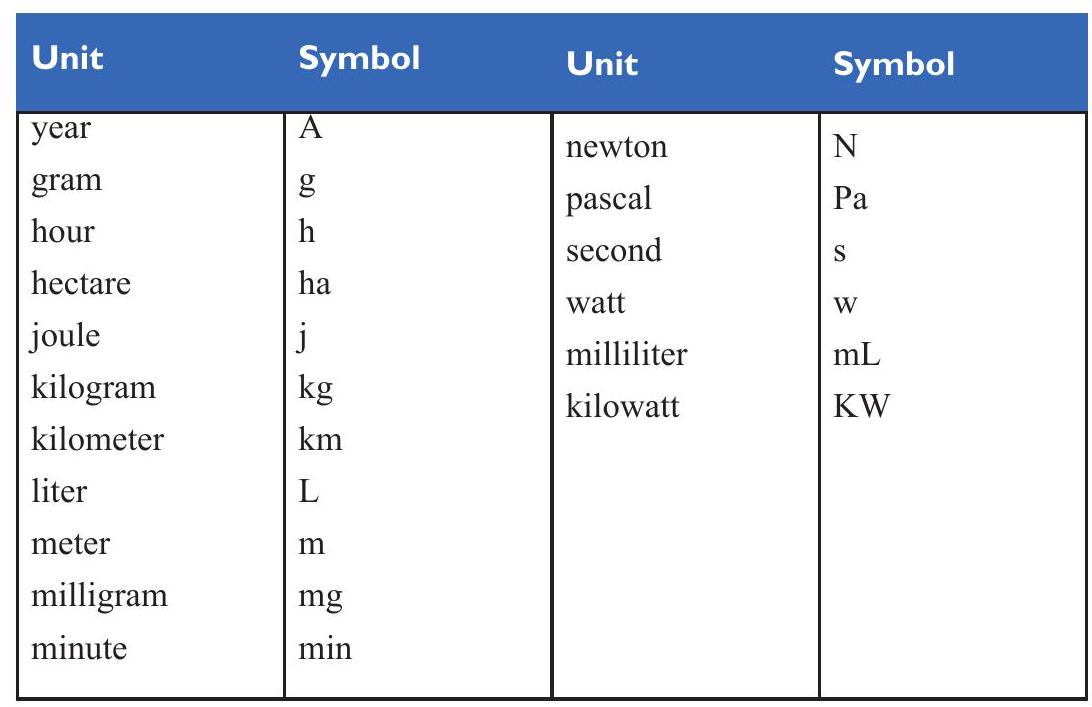
\includegraphics[max width=\textwidth]{2022_09_11_72dbedc910e6e984560cg-54}

\section{Metric to English Conversions}
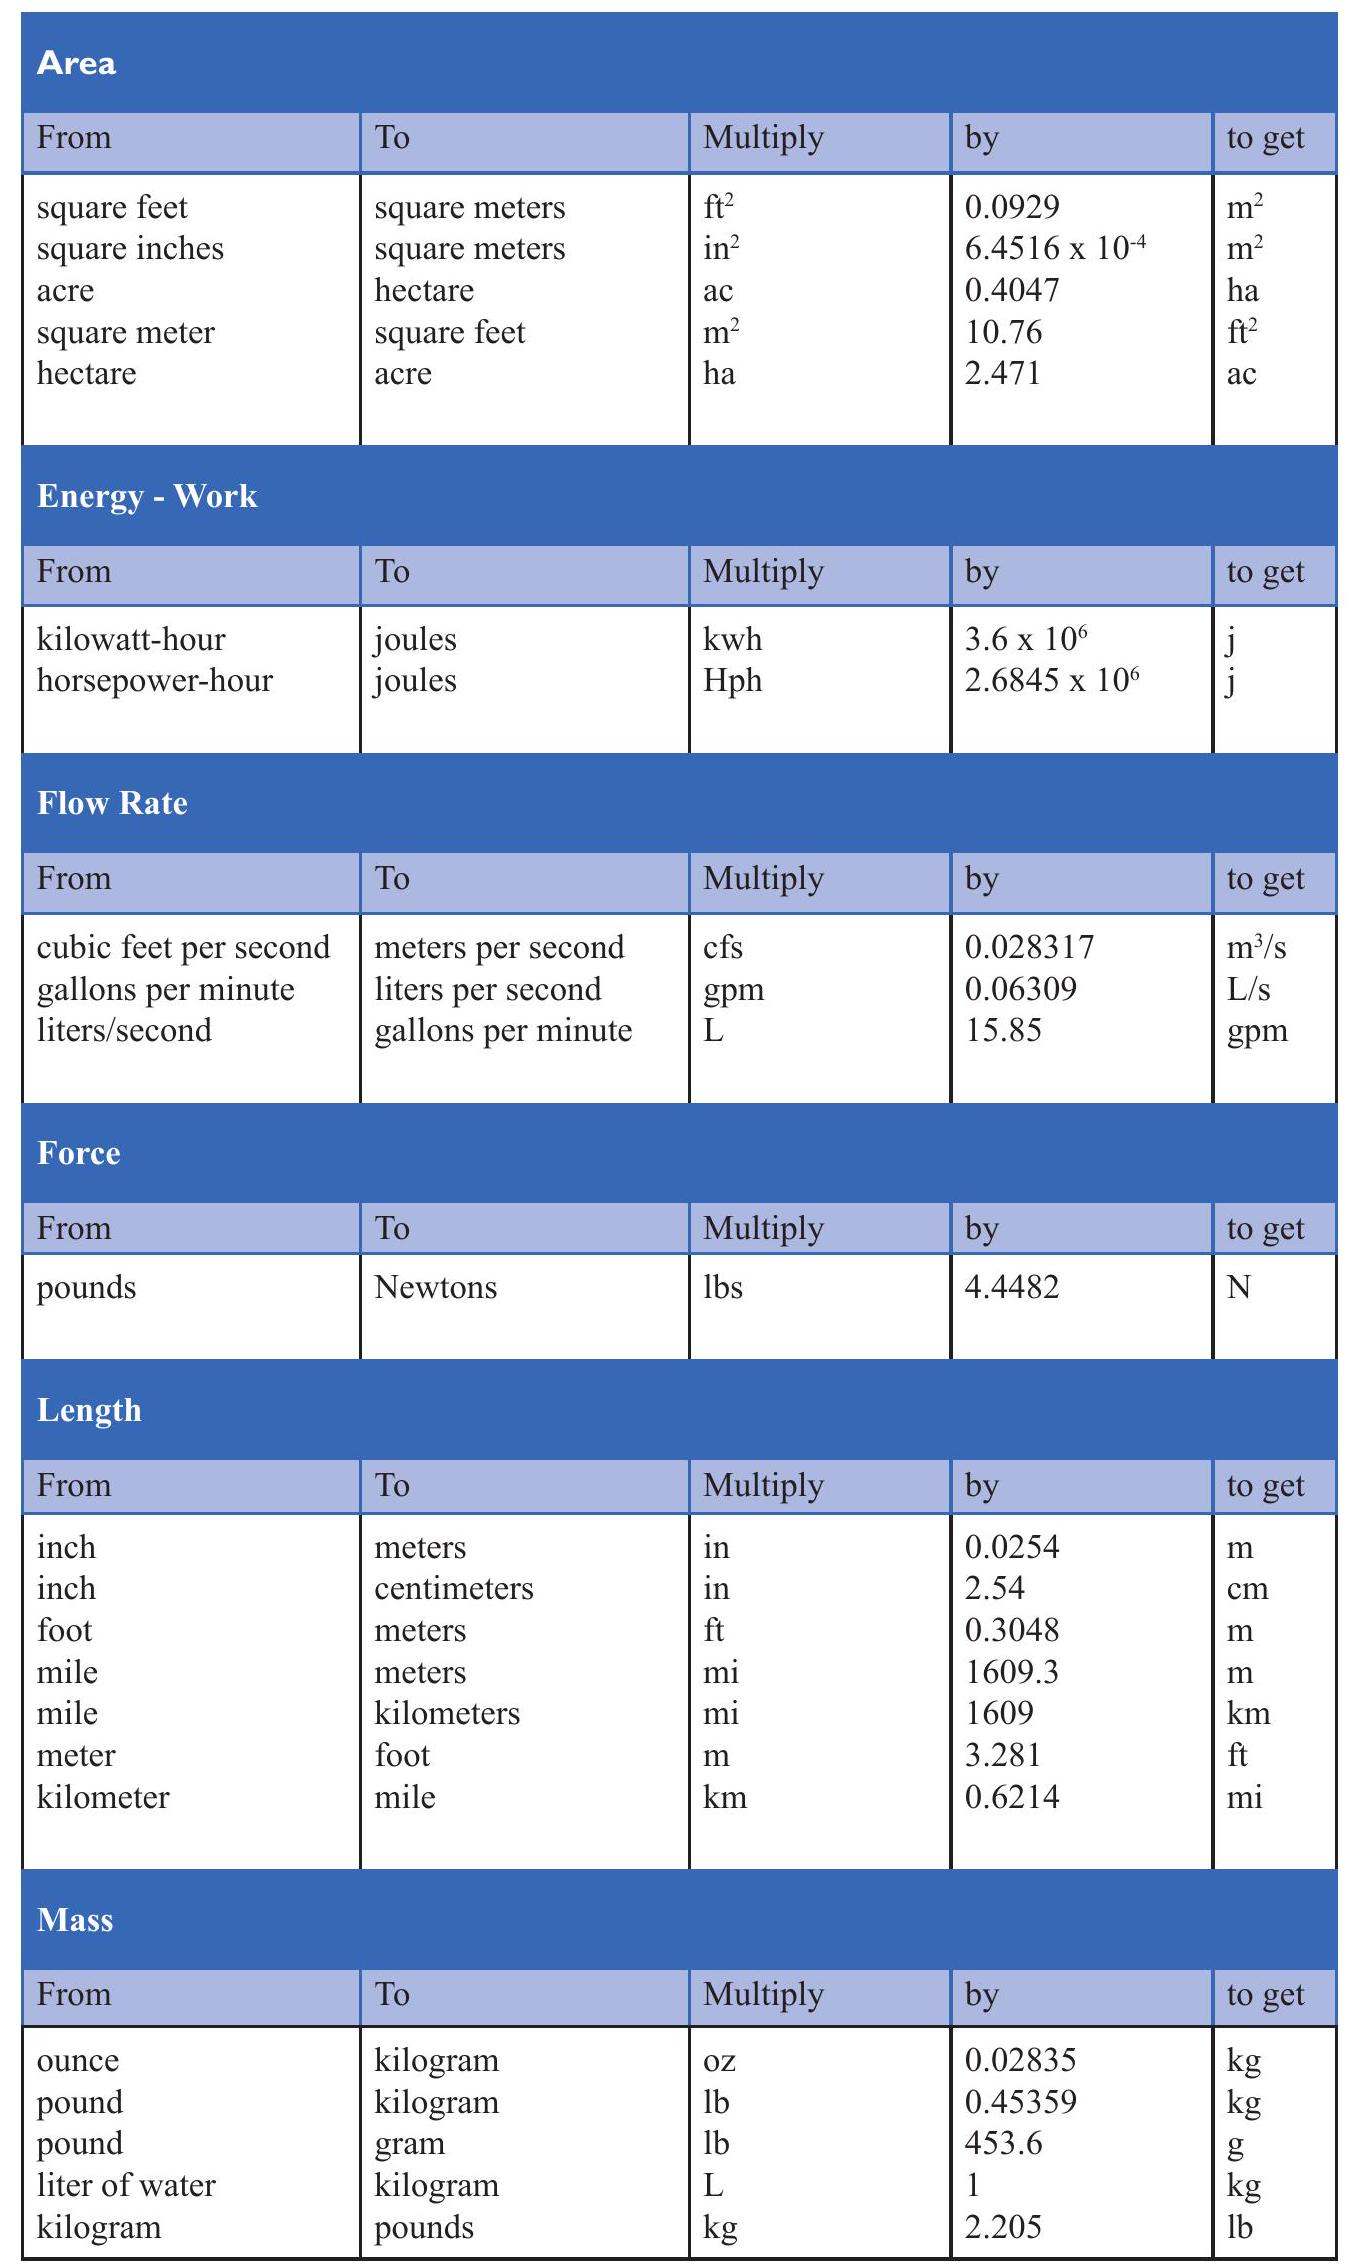
\includegraphics[max width=\textwidth]{2022_09_11_72dbedc910e6e984560cg-55}

\section{Metric to English Conversions}
\includegraphics[max width=\textwidth]{2022_09_11_72dbedc910e6e984560cg-56}

\section{Metric Conversions}
Two Types

Like the English system, there are two types of conversions: reducing or enlarging a value within the same base and converting between bases.

\section{Conversions in the Same Base}
Prefix Is the Key

The key to making conversions within the same base lies in understanding the prefixes and their associated values. For instance, the prefix kilo indicates 1000 ; therefore, a kilogram is 1000 grams, and a kilometer is 1000 meters.

\section{Linear Conversions}
The base unit of linear measurement is the meter. The common divisions of the meter are the following:

Kilometer $=1000$ meters

Centimeter $=1 / 100$ of a meter or there are 100 centimeters in a meter.

Millimeter $=1 / 1000$ of a meter or there are 1000 millimeters in a meter.

Example 1 - Conversion

Convert 4500 meters to kilometers.

Step 1 - Divide the number of meters by 1000 (kilo).

$\frac{4,500 \text { meters }}{1,000 \text { meters } / \text { kilometers }}=4.5$ kilometers

Example 2 - Conversion

Convert $4.6$ meters to centimeters.

Step 1 - Multiply meters times 100 (centi).

$4.6$ meters $x 100 \mathrm{~cm}=460 \mathrm{~cm}$

\section{Volume Conversions}
The most common volume conversion is from liters to milliliters. Since milli is the prefix for $0.001$, liters can be converted to milliliters by multiplying times 1000 .

Likewise, milliliters can be converted to liters by dividing by 1000 .

$1 \mathrm{~L}=1000 \mathrm{~mL}$

Example 3 - Conversion

Convert 2,400 mL to liters.

Step 1 - Divide the number of milliliters by 1000 .

$\frac{2,400 \mathrm{~mL}}{1,000 \mathrm{~mL} / \mathrm{L}}=2.4 \mathrm{~L}$

Example 4 - Conversion

Convert $0.35$ L to milliliters.

Step 1 - Multiply the number of liters times 1000 .

$0.35 \mathrm{~L} \mathrm{X} 1000 \mathrm{~mL} / \mathrm{L}=350 \mathrm{~mL}$

\section{Mass Conversion}
The two most common mass conversions are between kilograms and grams and between milligrams and grams. Since kilo is 1000 grams, it can be converted to kilograms by dividing by 1000 . Since milli is 1000 , grams can be converted to milligrams by multiplying by 1000 .

Example 5 - Conversion

Convert 2,600 mg to grams.

Step 1 - Divide the 2,600 mg by 1,000 .

$\frac{2,600 \mathrm{~g}}{1,000 \mathrm{mg} / \mathrm{g}}=2.6 \mathrm{~g}$

Example 6 - Conversion

Convert 1,345,000 g to kilograms.

Step 1 - Divide $1,345,000 \mathrm{~g}$ by 1,000 .
$$
\frac{1,345,000 \mathrm{~g}}{1,000 \mathrm{~g} / \mathrm{kg}}=1345 \mathrm{~kg}
$$

\section{Conversion to Another Base}
Key

The common conversion made between basic units is between mass and volume.

Volume in the metric system is expressed as liters, cubic meters, or cubic centimeters. The relationship between mass and volume is the following:

$1 \mathrm{~g}=1 \mathrm{ml}=1 \mathrm{cc}$, (one gram is equal to 1 milliliter is equal to 1 cubic centimeter)

Other Relationships

1 cubic meter $\left(\mathrm{m}^{3}\right)=1000$ liters

$1 \mathrm{~kg}=1 \mathrm{~L}$

\section{Cubic Measurements}
It is common practice to convert liters to cubic meters when the volume exceeds 1000 liters.

\section{Practice Problems - Answers}
Example 7 - Conversion

Convert 500 kilograms of water to liters.

Since kilograms and liters are the same base, the conversion is a simple matter of changing the units. $500 \mathrm{~kg}=500 \mathrm{~L}$

Example 8 - Conversion

Convert 3,600 L to cubic meters.

Step 1 - Divide the liters by 1000 .

$\frac{3,600 \mathrm{~L}}{1,000 \mathrm{~L} / \mathrm{m}^{3}}=3.6 \mathrm{~m}^{3}$

\section{Practice Problems - Metric Conversion}
A. Convert $4.2 \mathrm{~kg}$ to $\mathrm{g}$.

B. Convert $0.5 \mathrm{~kg}$ to g.

C. Convert $4600 \mathrm{~g}$ to $\mathrm{kg}$.

D. Convert $3.4 \mathrm{~km}$ to $\mathrm{m}$.

E. Convert $0.5 \mathrm{~km}$ to $\mathrm{m}$.

F. Convert $10,000 \mathrm{~m}$ to $\mathrm{km}$.

\section{Practice Problem Answers - Fractions}
\begin{enumerate}
  \item Reduce the following to their simplest terms.\\
A. 1/2 Both were divided by 2\\
B. 2/3 Both were divided by 6\\
C. 3/4 Is in its simplest terms\\
D. 3/4 Both were divided by 2\\
E. $3 / 4$ Both were divided by 8\\
F. 1/2 Both were divided by 9\\
G. $5 / 9$ Both were divided by 3
\end{enumerate}
\section{Practice Problem Answers - Rounding}
\begin{enumerate}
  \item Round the following to the nearest hundredths:\\
A. $2.4568=2.46$\\
B. $27.2534=27.25$\\
C. $128.2111=128.21$\\
D. $364.8762=364.88$\\
E. $354.777777=354.78$\\
F. $34.666666=34.67$\\
G. $67.33333=67.33$

  \item Round the following answers off to the most significant digit:\\
A. $26.34 \times 124.34567=3,275.26495=3,275.26$\\
B. $25.1+26.43=51.53$\\
$=51.5$\\
C. $128.456-121.4=7.056$\\
$=7.1$\\
D. $23.5 \mathrm{ft} \times 34.25 \mathrm{ft}=804.875 \mathrm{ft}^{2}$\\
$=804.9 \mathrm{ft}^{2}$\\
E. $12,457.92 \times 3=37,373.76$\\
$=37,374$

\end{enumerate}
\section{Practice Problem Answer - Averages}
\begin{enumerate}
  \item The total is $2.4$. There are 9 numbers in the set. Therefore $2.4 \div 9=0.2667$, rounding to $0.3$.
\end{enumerate}
\section{Practice Problem Answers - Formulas}
\begin{enumerate}
  \item Find the diameter of a settling basin that has a circumference of 126 feet.
\end{enumerate}
$$
\begin{aligned}
&\mathrm{C}=\pi \mathrm{D} \\
&126 \mathrm{ft}=\pi \mathrm{D} \\
&\mathrm{D}=\frac{126 \mathrm{ft}}{\pi}=40 \mathrm{ft}
\end{aligned}
$$

\begin{enumerate}
  \setcounter{enumi}{2}
  \item Find the diameter of a pipe that has a circumference of $129 / 16 "$.
\end{enumerate}
$$
\begin{aligned}
&129 / 16 "=12.56 " \\
&\mathrm{C}=\pi \mathrm{D} \\
&12.56 \mathrm{in}=\pi \mathrm{D} \\
&\mathrm{D}=\frac{12.56 \mathrm{in}}{\pi}=4 \text { in }
\end{aligned}
$$

\begin{enumerate}
  \setcounter{enumi}{3}
  \item Find the diameter of a settling basin that has a surface area of $113 \mathrm{ft}^{2}$.
\end{enumerate}
$$
\begin{aligned}
&\mathrm{A}=\pi \mathrm{r}^{2} \\
&113 \mathrm{ft}^{2}=\pi \mathrm{r}^{2} \\
&\mathrm{r}=\sqrt{\frac{113 \mathrm{ft}}{\pi}}=5.997 \text { or } 6 \mathrm{ft} \\
&6 \mathrm{ft} \times 2=12 \mathrm{ft} \text { diameter }
\end{aligned}
$$

\begin{enumerate}
  \setcounter{enumi}{4}
  \item Find the diameter of a storage tank that has a surface area of $314 \mathrm{ft}^{2}$.
\end{enumerate}
$$
\begin{aligned}
&\mathrm{A}=\pi \mathrm{r}^{2} \\
&314 \mathrm{ft}^{2}=\pi \mathrm{r}^{2} \\
&\mathrm{r}=\sqrt{\frac{113 \mathrm{ft}}{\pi}}=9.997 \text { or } 10 \mathrm{ft} \\
&\mathrm{D}=10 \mathrm{ft} \times 2=20 \mathrm{ft}
\end{aligned}
$$

\begin{enumerate}
  \setcounter{enumi}{5}
  \item The detention time in a chlorine contact chamber is 42 minutes. If the chamber holds 3200 gallons, what is the flow rate in gpm?
\end{enumerate}
$$
\begin{aligned}
&\mathrm{DT}=\frac{\text { Volume }}{\text { Flow }} \\
&42 \mathrm{~min}=\frac{3200 \mathrm{gal}}{\text { flow, gpm }}=\text { flow, gpm }=\frac{3200 \mathrm{gal}}{42 \mathrm{~min}} \\
&\text { flow }=76 \mathrm{gpm}
\end{aligned}
$$

\begin{enumerate}
  \setcounter{enumi}{6}
  \item A clearwell has a detention time of 2 hours. What is the flow rate in gpm if the clarifier holds 8000 gallons?
\end{enumerate}
$$
\begin{aligned}
&\mathrm{DT}=\frac{\text { Volume }}{\text { Flow }} \\
&120 \mathrm{~min}=\frac{8000 \mathrm{gal}}{\text { flow, gpm }}=\text { flow, gpm }=\frac{8000 \mathrm{gal}}{120 \mathrm{~min}}
\end{aligned}
$$
flow, $\mathrm{gpm}=67 \mathrm{gpm}$

\begin{enumerate}
  \setcounter{enumi}{7}
  \item A rectangular settling basin has a weir length of 10 feet. What is the weir overflow rate when the flow is $80,000 \mathrm{gpd}$ ?
\end{enumerate}
$$
\begin{aligned}
&\mathrm{WO}=\frac{\text { Flow rate in gpd }}{\text { Weir length in feet }} \\
&\mathrm{WO}=\frac{80,000 \mathrm{gpd}}{10 \mathrm{ft}}=8,000 \mathrm{gpd} / \mathrm{ft}
\end{aligned}
$$

\section{Practice Problem Answers - Perimeter/Circumference}
\begin{enumerate}
  \item Find the perimeter or circumference of the following items:\\
A. $=\pi \times 14$ inches $=44$ inches\\
B. $6 \mathrm{ft}+9 \mathrm{ft}+6 \mathrm{ft}+9 \mathrm{ft}=30 \mathrm{ft}$\\
C. $42 \mathrm{ft}+20 \mathrm{ft}+42 \mathrm{ft}+20 \mathrm{ft}=124 \mathrm{ft}$\\
D. $\pi \times 28$ feet $=88$ feet
\end{enumerate}
\section{Practice Problem Answers - Area}
\begin{enumerate}
  \item Find the area of the following items:\\
A. Diameter is 14 inches. Therefore, the radius, being $1 / 2$ of the diameter, is 7 inches.\\
$\mathrm{A}=\pi \times(7 \text { in })^{2}$\\
$\mathrm{A}=\pi \times 49 \mathrm{in}^{2}$\\
$\mathrm{A}=154 \mathrm{in}^{2}$\\
B. $\mathrm{A}=\mathrm{L} \times \mathrm{W}$\\
$\mathrm{A}=9 \mathrm{ft} \times 6 \mathrm{ft}=54 \mathrm{ft}^{2}$\\
C. $\mathrm{A}=\mathrm{L} x \mathrm{~W}$\\
$A=42 \mathrm{ft} \times 20 \mathrm{ft}$\\
$\mathrm{A}=840 \mathrm{ft}^{2}$\\
D. The diameter is 28 feet. The radius is one-half of the diameter; therefore, the radius is 14 feet.\\
$A=\pi \times r^{2}$\\
$\mathrm{A}=\pi \mathrm{x}(14 \mathrm{feet})^{2}$\\
$\mathrm{A}=\pi \times 196 \mathrm{ft}^{2}$\\
$\mathrm{A}=616 \mathrm{ft}^{2}$
\end{enumerate}
\section{Practice Problem Answers - Volume}
\begin{enumerate}
  \item Find the volume of the following:
\end{enumerate}
A. 3-inch pipe 200 feet long

\includegraphics[max width=\textwidth]{2022_09_11_72dbedc910e6e984560cg-63}

Hint: change the diameter of the pipe from inches to feet by dividing by $12 .$

\begin{enumerate}
  \item Change diameter to feet $3 \div 12=0.25 \mathrm{ft}$.

  \item Find the radius by dividing the diameter by 2 .

\end{enumerate}
$0.25 \mathrm{ft} \div 2=0.125 \mathrm{ft}$

\begin{enumerate}
  \setcounter{enumi}{3}
  \item Find the volume.
\end{enumerate}
$\mathrm{V}=\mathrm{L} x \pi \mathrm{r}^{2}$

$\mathrm{V}=200 \mathrm{ft} x \pi(0.125 \mathrm{ft})^{2}$

$\mathrm{V}=200 \mathrm{ft} \mathrm{x} \pi \mathrm{x} 0.01563 \mathrm{ft}^{2}$

$\mathrm{V}=9.8 \mathrm{ft}^{3}$

B. Find the volume of a fuel tank 4 feet in diameter and 10 feet long.

\includegraphics[max width=\textwidth]{2022_09_11_72dbedc910e6e984560cg-63(1)}

\begin{enumerate}
  \item Find the radius of the tank. The radius is one-half of the diameter. $4 \mathrm{ft} \div 2=2 \mathrm{ft}$

  \item Find the volume.

\end{enumerate}
$\mathrm{V}=\mathrm{L} x \pi \mathrm{r}^{2}$

$\mathrm{V}=10 \mathrm{ft} \mathrm{x} \pi(2 \mathrm{ft})^{2}$

$\mathrm{V}=10 \mathrm{ft} \mathrm{x} \pi \mathrm{x} 4 \mathrm{ft}^{2}$

$\mathrm{V}=125.7 \mathrm{ft}^{3}$ C. Find the volume of a chlorine barrel that is 20 inches in diameter and 42 inches tall.

\includegraphics[max width=\textwidth]{2022_09_11_72dbedc910e6e984560cg-64}

\begin{enumerate}
  \item Find the radius of the tank. The radius is one-half of the diameter. 20 inches $\div 2=10$ inches

  \item Find the volume.

\end{enumerate}
$\mathrm{V}=\mathrm{H} \times \pi \mathrm{r}^{2}$

$\mathrm{V}=42$ in $\mathrm{x} \pi(10 \mathrm{in})^{2}$

$\mathrm{V}=42$ in $\mathrm{x} \pi \times 100$ in $^{2}$

$\mathrm{V}=13,195 \mathrm{in}^{3}$

D. Find the volume of a trench $2.5$ feet wide, 6 feet deep, and 60 feet long.

\includegraphics[max width=\textwidth]{2022_09_11_72dbedc910e6e984560cg-64(1)}

$\mathrm{V}=\mathrm{L} \times \mathrm{W} \times \mathrm{D}$

$\mathrm{V}=60 \mathrm{ft} \times 2.5 \mathrm{ft} \times 6 \mathrm{ft}$

$\mathrm{V}=900 \mathrm{ft}^{3}$

\section{Practice Problem Answers - Percentage}
A. $25 \%$ of the chlorine in a 30 gallon vat has been used. How many gallons are remaining in the vat?

\begin{enumerate}
  \item Find the percentage of chlorine remaining.
\end{enumerate}
$100 \%-25 \%=75 \%$

\begin{enumerate}
  \setcounter{enumi}{2}
  \item Change the percent to a decimal.
\end{enumerate}
$75 \% \div 100=0.75$

\begin{enumerate}
  \setcounter{enumi}{3}
  \item Multiply the percent as a decimal times the tank volume.
\end{enumerate}
$0.75 \times 30 \mathrm{gal}=22.5 \mathrm{gal}$

B. The annual public works budget is $\$ 147,450.00$. If $75 \%$ of the budget should be spent by the end of September, how many dollars are to be spent? How much is remaining?

\begin{enumerate}
  \item Change the percentage to a decimal.
\end{enumerate}
$75 \% \div 100=0.75$

\begin{enumerate}
  \setcounter{enumi}{2}
  \item Multiply the budget amount by the percent to be used.
\end{enumerate}
$\$ 147,450.00 \times 0.75=\$ 110,587.50$ to be spent

\begin{enumerate}
  \setcounter{enumi}{3}
  \item Find what will be remaining.
\end{enumerate}
$\$ 147,450.00-110,587.50=\$ 36,862.50$

C. There are 50 pounds of pure chlorine in a container of $67 \%$ calcium hypochlorite.

What is the total weight of the container?

\begin{enumerate}
  \item Change the percent to a decimal.
\end{enumerate}
$67 \% \div 100=0.67$

\begin{enumerate}
  \setcounter{enumi}{2}
  \item Divide the weight by the percentage.
\end{enumerate}
$\frac{50 \mathrm{lbs}}{0.67}=74.6 \mathrm{lbs}$

D. $3 / 4$ is the same as what percentage?

\begin{enumerate}
  \item Change the fraction into a decimal.
\end{enumerate}
$$
\frac{3}{4}=0.75
$$

\begin{enumerate}
  \setcounter{enumi}{2}
  \item Convert to a percentage.
\end{enumerate}
$0.75 \times 100=75 \%$

E. A $2 \%$ chlorine solution is what concentration in $\mathrm{mg} / \mathrm{L}$ ?

\begin{enumerate}
  \item Change the percentage to a decimal.
\end{enumerate}
$2 \% \div 100=0.02$

\begin{enumerate}
  \setcounter{enumi}{2}
  \item Multiply times one million.
\end{enumerate}
$0.02 \times 1,000,000=20,000 \mathrm{mg} / \mathrm{L}$ F. A water plant produces 84,000 gallons per day. 7,560 gallons are used to backwash the filter. What percentage of water is used to backwash?

\begin{enumerate}
  \item Divide the part by the whole.
\end{enumerate}
$$
\frac{7,560 \text { gal }}{84,000 \text { gal }}=0.09
$$

\begin{enumerate}
  \setcounter{enumi}{2}
  \item Change the value to a percentage.
\end{enumerate}
$0.09 \times 100=9 \%$

G. The average day winter demand of a community is 14,500 gallons. If the summer demand is estimated to be $72 \%$ greater than the winter, what is the estimated summer demand?

\begin{enumerate}
  \item Change the percent to a decimal.
\end{enumerate}
$72 \% \div 100=0.72$

\begin{enumerate}
  \setcounter{enumi}{2}
  \item Add this value to 1 .
\end{enumerate}
$1+0.72=1.72$

\begin{enumerate}
  \setcounter{enumi}{3}
  \item Multiply the demand times this value.
\end{enumerate}
14,500 gal x $1.72=24,940$ gal

\section{Practice Problem Answers - Efficiency}
A. The water horsepower of a pump is $10 \mathrm{Hp}$ and the brake horsepower output of the motor is $15.4 \mathrm{Hp}$. What is the efficiency of the motor?

$\frac{10 \mathrm{BHp}}{15.4 \mathrm{EHp}} \times 100=64.94$ or $65 \%$

B. The water horsepower of a pump is $25 \mathrm{Hp}$ and the brake horsepower output of the motor is $48 \mathrm{Hp}$. What is the efficiency of the motor?

$\frac{25 \mathrm{BHp}}{48 \mathrm{EHp}} \times 100=52 \%$

C. The efficiency of a well pump is determined to be $75 \%$. The efficiency of the motor is estimated at $94 \%$. What is the efficiency of the well?

$0.75 \times 0.94=0.705 \times 100=70.5 \%$

D. If a motor is $85 \%$ efficient and the output of the motor is determined to be 10

$\mathrm{BHp}$, what is the electrical horsepower requirement of the motor?

$\frac{10 \mathrm{BHp}}{0.85}=11.8 \mathrm{EHp}$ E. The water horsepower of a well with a submersible pump has been calculated at 8.2 WHp. The Output of the electric motor is measured as $10.3 \mathrm{BHp}$. What is the efficiency of the pump?

$\frac{82 \mathrm{WHp}}{10.3 \mathrm{BHp}} \times 100=79.6 \%$

\section{Practice Problem Answers - Conversion}
\begin{enumerate}
  \item Convert the following:
\end{enumerate}
A. $750 \mathrm{ft}^{3}$ of water to gallons
$$
\begin{aligned}
&750 \frac{\mathrm{ft}^{3}}{1} \times \frac{?}{\mathrm{ft}^{3}}= \\
&750 \frac{\mathrm{ft}^{3}}{1} \times \frac{\mathrm{gal}}{\mathrm{ft}^{3}}= \\
&750 \frac{\mathrm{ft}^{3}}{1} \times \frac{7.48 \mathrm{gal}}{\mathrm{ft}^{3}}=5,610 \mathrm{gal}
\end{aligned}
$$
B. 50 gallons to pounds
$$
\begin{aligned}
&50 \frac{\text { gal }}{1} \times \frac{?}{\text { gal }}= \\
&50 \frac{\text { gal }}{1} \times \frac{1 \mathrm{lbs}}{\text { gal }}= \\
&50 \frac{\text { gal }}{1} \times \frac{8.34 \mathrm{lbs}}{\text { gal }}=417 \mathrm{lbs}
\end{aligned}
$$
C. 560 gpm to $\mathrm{cfs}$
$$
\begin{aligned}
& 560 \frac{\mathrm{gpm}}{1} \times \frac{?}{\mathrm{gpm}}= \\
& 560 \frac{\mathrm{gpm}}{1} \times \frac{1 \mathrm{cfs}}{448 \mathrm{gpm}}=1.25 \mathrm{cfs}
\end{aligned}
$$
\includegraphics[max width=\textwidth]{2022_09_11_72dbedc910e6e984560cg-67}

D. $4 \mathrm{lbs}$ to ounces
$$
\begin{aligned}
& 4 \frac{\mathrm{lbs}}{1} \times \stackrel{?}{\mathrm{lbs}}= \\
& 4 \frac{\mathrm{lbs}}{1} \times \stackrel{\mathrm{oz}}{\mathrm{lbs}}= \\
& 4 \frac{\mathrm{lbs}}{1} \times \frac{16 \mathrm{oz}}{\mathrm{lbs}}=64 \mathrm{oz}
\end{aligned}
$$
E. $128 \mathrm{ft}^{3}$ of water to weight in pounds
$$
\begin{aligned}
&128 \frac{\mathrm{ft}^{3}}{1} \times \frac{?}{\mathrm{ft}^{3}}= \\
&128 \frac{\mathrm{ft}^{3}}{1} \times \frac{\mathrm{lbs}}{\mathrm{ft}^{3}}= \\
&128 \frac{\mathrm{ft}^{3}}{1} \times \frac{62.4 \mathrm{lbs}}{\mathrm{ft}^{3}}=7,987 \mathrm{lbs}
\end{aligned}
$$
G. $3.4 \mathrm{cfs}$ to gpm
$$
\begin{aligned}
& 340 \frac{\mathrm{cfs}}{1} \times \longrightarrow \frac{?}{\mathrm{cfs}}= \\
& 340 \frac{\mathrm{cfs}}{1} \times \stackrel{\mathrm{gpm}}{\mathrm{cfs}}= \\
& 340 \frac{\mathrm{cfs}}{1} \times \frac{448 \mathrm{gpm}}{1 \mathrm{cfs}}=1,523 \mathrm{gpm}
\end{aligned}
$$
H. $65 \mathrm{ft}^{3}$ to $\mathrm{yd}^{3}$
$$
65 \frac{\mathrm{ft}^{3}}{1} \times \frac{1 \mathrm{yd}^{3}}{27 \mathrm{ft}^{3}}=2.4 \mathrm{yd}^{3}
$$
I. 3,000 gallons to $\mathrm{ft}^{3}$
$$
3,000 \frac{\text { gal }}{1} \times \frac{1 \mathrm{ft}^{3}}{7.48 \mathrm{gal}}=401 \mathrm{ft}^{3}
$$
J. 250,000 gallons to $\mathrm{MG}$
$$
250,000 \frac{\text { gal }}{1} \times \frac{1 \mathrm{MG}}{1,000,000 \mathrm{gal}}=0.25 \mathrm{MG}
$$
$$
\begin{aligned}
&\text { K. } 75 \text { gpm to MGD } \\
&75 \text { gpm x } 1440 \mathrm{~min} / \text { day }=108,000 \mathrm{gpd} \\
&108,000 \frac{\text { gpd }}{1} \times \frac{1 \mathrm{MGD}}{1,000,000 \mathrm{gpd}}=0.108 \mathrm{MGD}
\end{aligned}
$$
L. 8 inches to feet
$$
8 \frac{\text { in }}{1} \times \frac{1 \mathrm{ft}}{12 \text { in }}=0.667 \mathrm{ft}
$$
M. 2.4 MGD to $\mathrm{cfs}$
$$
\begin{aligned}
&2.4 \frac{\mathrm{MGD}}{1} \times \frac{1,000,000 \mathrm{gpd}}{1 \mathrm{MGD}}=2,400,000 \mathrm{gpd} \\
&2,400,000 \frac{\mathrm{gal}}{\text { day }} \times \frac{1 \mathrm{day}}{1,440 \mathrm{~min}}=1,667 \mathrm{gpm} \\
&1,667 \frac{\mathrm{gpm}}{1} \times \frac{1 \mathrm{cfs}}{448 \mathrm{gpm}}=3.7 \mathrm{cfs}
\end{aligned}
$$
N. 2.4 MGD to gpm
$$
2.4 \frac{\mathrm{MGD}}{1} \times \frac{694.5 \mathrm{gpm}}{1 \mathrm{MGD}}=1,668.8 \mathrm{cfs}
$$
O. 65 pints to gallons
$$
65 \frac{\text { pint }}{1} \times \frac{1 \mathrm{gal}}{8 \text { pint }}=8.125 \mathrm{gal}
$$
P. $2.5 \mathrm{ft}^{2}$ to square inches
$$
2.5 \frac{\mathrm{ft}^{2}}{1} \times \frac{144 \mathrm{in}^{2}}{1 \mathrm{ft}^{2}}=360 \mathrm{in}^{2}
$$
Q. 7 yards to feet
$$
7 \frac{\mathrm{yd}}{1} \times \frac{3 \mathrm{ft}}{1 \mathrm{yd}}=21 \mathrm{ft}
$$
R. 36,000 gpd to gpm
$$
36,000 \frac{\mathrm{gpd}}{1} \times \frac{\mathrm{gpm}}{1,440 \mathrm{gpd}}=25 \mathrm{gpm}
$$
S. $125 \mathrm{gpm}$ to $\mathrm{gph}$

$125 \mathrm{gpm} \times 60 \mathrm{~min} / \mathrm{hr}=7,500 \mathrm{gph}$

\section{Practice Problem Answers - Temperature Conversion}
A. Change $70^{\circ} \mathrm{F}$ to ${ }^{\circ} \mathrm{C}$
$$
{ }^{\circ} \mathrm{C}=\frac{70^{\circ} \mathrm{F}-32^{\circ}}{1.8}=21^{\circ} \mathrm{C}
$$
B. Change $140^{\circ} \mathrm{F}$ to ${ }^{\circ} \mathrm{C}$
$$
\begin{aligned}
&{ }^{\circ} \mathrm{C}=\frac{140^{\circ} \mathrm{F}-32^{\circ}}{1.8}=60^{\circ} \mathrm{C} \\
&\text { C. Change } 20^{\circ} \mathrm{C} \text { to }{ }^{\circ} \mathrm{F} \\
&{ }^{\circ} \mathrm{F}={ }^{\circ} \mathrm{C} \times 1.8+32^{\circ} \\
&{ }^{\circ} \mathrm{F}=20^{\circ} \mathrm{C} \times 1.8+32^{\circ} \\
&{ }^{\circ} \mathrm{F}=68^{\circ} \mathrm{F} \\
&\text { D. Change } 85^{\circ} \mathrm{C} \text { to }{ }^{\circ} \mathrm{F} \\
&{ }^{\circ} \mathrm{F}={ }^{\circ} \mathrm{C} \times 1.8+32^{\circ} \\
&{ }^{\circ} \mathrm{F}=85^{\circ} \mathrm{C} \times 1.8+32^{\circ} \\
&{ }^{\circ} \mathrm{F}=185^{\circ} \mathrm{F} \\
&\text { E. Change } 4{ }^{\circ} \mathrm{C} \text { to }{ }^{\circ} \mathrm{F} \\
&{ }^{\circ} \mathrm{F}={ }^{\circ} \mathrm{C} \times 1.8+32^{\circ} \\
&{ }^{\circ} \mathrm{F}=4^{\circ} \mathrm{C} \times 1.8+32^{\circ} \\
&{ }^{\circ} \mathrm{F}=39^{\circ} \mathrm{F}
\end{aligned}
$$

\section{Practice Problem Answers - Pressure and Head}
\begin{enumerate}
  \item Make the following conversions:
\end{enumerate}
A. Convert a pressure of 45 psi to feet of head.
$$
45 \frac{\mathrm{psi}}{1} \times \frac{\mathrm{ft}}{0.433 \mathrm{psi}}=103.9 \text { feet }
$$
B. Convert 12 psi to feet.
$$
12 \frac{\mathrm{psi}}{1} \times \frac{\mathrm{ft}}{0.433 \mathrm{psi}}=27.7 \text { feet }
$$
C. Convert $85 \mathrm{psi}$ to feet.
$$
85 \frac{\mathrm{psi}}{1} \times \frac{\mathrm{ft}}{0.433 \mathrm{psi}}=196.3 \text { feet }
$$
D. It is 112 feet in elevation between the top of the reservoir and the watering point. What will the static pressure be at the watering point?
$$
112 \frac{\mathrm{ft}}{1} \times \frac{0.433 \mathrm{psi}}{1 \mathrm{ft}}=48.5 \text { feet }
$$
E. A reservoir is 20 feet deep. What will the pressure be at the bottom of the reservoir?
$$
20 \frac{\mathrm{ft}}{1} \mathrm{x} \frac{0.433 \mathrm{psi}}{1 \mathrm{ft}}=8.7 \text { feet }
$$

\section{Practice Problem Answers - Flow}
A. Find the flow in MGD when the flow is $34,000 \mathrm{gpd}$.
$$
\frac{34,000 \text { gpd }}{1,000,000}=0.034 \mathrm{MGD}
$$
B. Find the flow in gpm when the total flow for the day is $65,000 \mathrm{gpd}$.
$$
\frac{65,000 \mathrm{gpd}}{1,440 \mathrm{~min} / \mathrm{day}}=45 \mathrm{gpm}
$$
C. Find the flow in gpm when the flow is $1.3 \mathrm{cfs}$.
$$
1.3 \frac{\mathrm{cfs}}{1} \mathrm{x} \frac{448 \mathrm{gpm}}{1 \mathrm{cfs}}=582 \mathrm{gpm}
$$
D. Find the flow in gpm when the flow is $0.25 \mathrm{cfs}$.
$$
0.25 \frac{\mathrm{cfs}}{1} \times \frac{448 \mathrm{gpm}}{1 \mathrm{cfs}}=112 \mathrm{gpm}
$$
E. Find the flow in a 4-inch pipe when the velocity is $1.5$ feet per second.

The diameter of the pipe is 4 inches. Therefore, the radius is 2 inches. Convert the 2 inches to feet.
$$
\begin{aligned}
&\frac{2}{12}=0.6667 \mathrm{ft} \\
&\mathrm{A}=\pi \times \mathrm{r}^{2} \\
&\mathrm{~A}=\pi \times(0.167 \mathrm{ft})^{2} \\
&\mathrm{~A}=\pi \times 0.028 \mathrm{ft}^{2} \\
&\mathrm{~A}=0.09 \mathrm{ft}^{2} \\
&\mathrm{Q}=\mathrm{V} \times \mathrm{A} \\
&\mathrm{Q}=1.5 \mathrm{ft} / \mathrm{sec} \times 0.09 \mathrm{ft}^{2} \\
&\mathrm{Q}=0.14 \mathrm{ft} / 3 \mathrm{sec}(\mathrm{cfs})
\end{aligned}
$$

\section{Practice Problem Answers - Detention Time}
A. How long will it take to fill a 50 gallon hypochlorite tank if the flow is $5 \mathrm{gpm}$ ?
$$
\frac{50 \mathrm{gal}}{5 \mathrm{gal} / \mathrm{min}}=10 \mathrm{~min}
$$
B. Find the detention time in a 45,000 gallon reservoir if the flow rate is $85 \mathrm{gpm}$.
$$
\mathrm{DT}=\frac{45,000 \mathrm{gal}}{85 \mathrm{gal} / \mathrm{min}}=529 \mathrm{~min} \quad \text { or } \frac{529 \mathrm{~min}}{60 \mathrm{~min} / \mathrm{hr}}=8.8 \mathrm{hrs}
$$
C. If the fuel consumption to the boiler is 35 gallons per day. How many days will the 500 gallon tank last.
$$
\text { Days }=\frac{500 \text { gal }}{35 \mathrm{gal} / \text { day }}=14.3 \text { days }
$$
D. The sedimentation basin on a water plant contains 5,775 gallons. What is the detention time if the flow is $175 \mathrm{gpm}$.
$$
\mathrm{DT}=\frac{5,775 \mathrm{gal}}{175 \mathrm{gal} / \mathrm{min}}=33 \mathrm{~min}
$$

\section{Practice Problem Answers - Ratio and Proportion}
A. It takes 6 gallons of chlorine solution to obtain a proper residual when the flow is 45,000 gpd. How many gallons will it take when the flow is 62,000 gpd?
$$
\frac{6 \text { gallons }}{\text { X gallons }}: \begin{aligned}
&45,000 \mathrm{gpd} \\
&62,000 \mathrm{gpd}
\end{aligned}
$$
$(\mathrm{X}$ gallons $)(45,000 \mathrm{gpd})=(6$ gallons $)(62,000 \mathrm{gpd})$
$$
\mathrm{X} \mathrm{gal}=\frac{(6 \mathrm{gal})(62,000 \mathrm{gpd})}{62,000 \mathrm{gpd}}=8.3 \mathrm{gal}
$$
B. A motor is rated at $41 \mathrm{amps}$ average draw per leg at $30 \mathrm{Hp}$. What is the actual $\mathrm{Hp}$ when the draw is $36 \mathrm{amps}$ ?
$$
\begin{aligned}
&\frac{41 \mathrm{amps}}{36 \mathrm{amps}}: \begin{array}{l}
30 \mathrm{Hp} \\
\mathrm{XHp}
\end{array} \\
&(41 \mathrm{amps})(\mathrm{X} \mathrm{Hp})=(36 \mathrm{amps})(30 \mathrm{Hp}) \\
&\text { X Hp }=\frac{(36 \mathrm{amps})(30 \mathrm{Hp})}{41 \mathrm{amps}}=26.3 \mathrm{Hp}
\end{aligned}
$$
C. It it takes 2 operators $4.5$ days to clean an aeration basin, how long will it take three operators to do the same job?
$$
\begin{aligned}
&\frac{2 \text { operators }}{3 \text { operators }}: \quad \mathrm{X} \text { days } \\
&4.5 \text { days } \\
&(2 \text { operators })(\mathrm{X} \text { days })=(3 \text { operators })(4.5 \text { days }) \\
&\mathrm{X} \text { days }=\frac{(2 \text { operators })(4.5 \text { days })}{3 \text { operators }}=3 \text { days }
\end{aligned}
$$
D. If it takes 20 minutes to pump a wet well down with one pump pumping at 125 gpm, then how long will it take if a 200 gpm pump is used?
$$
\begin{aligned}
&\frac{20 \mathrm{~min}}{\mathrm{Xmin}}: \quad \begin{array}{l}
200 \mathrm{gpm} \\
125 \mathrm{gpm}
\end{array} \\
&(\mathrm{Xmin})(200 \mathrm{gpm})=(20 \mathrm{~min})(125 \mathrm{gpm}) \\
&\mathrm{Xmin}=\frac{(20 \mathrm{~min})(125 \mathrm{gpm})}{200 \mathrm{gpm}}=12.5 \mathrm{~min}
\end{aligned}
$$
E. It takes 3 hours to clean 400 feet of collection system using a sewer ball. How long will it take to clean 250 feet?
$$
\frac{3 \mathrm{hrs}}{\mathrm{Xhrs}}: \begin{gathered}
400 \mathrm{ft} \\
250 \mathrm{ft}
\end{gathered}
$$
$(\mathrm{X} \mathrm{hrs})(400 \mathrm{ft})=(3 \mathrm{hrs})(250 \mathrm{ft})$

\includegraphics[max width=\textwidth]{2022_09_11_72dbedc910e6e984560cg-73}

F. It takes 14 cups of $\mathrm{HTH}$ to make a $12 \%$ solution. Each cup holds 300 grams, how many cups will it take to make a $5 \%$ solution?
$$
\begin{aligned}
&\frac{14 \text { cups }}{X \text { cups }}: \quad 12 \% \\
&\text { (X cups })(12 \%)=(14 \text { cups })(5 \%) \\
&\text { X cups }=\frac{(14 \text { cups })(5 \%)}{12 \%}=5.8 \text { cups }
\end{aligned}
$$

\section{Practice Problem Answers - Pounds Formula}
A. How many pounds of $100 \%$ gas chlorine are needed to disinfect a flow of 85,000 gpd at $12 \mathrm{mg} / \mathrm{L}$ ?\\
$\mathrm{lbs}=0.085 \mathrm{MGD} \times 8.34 \mathrm{lbs} / \mathrm{gal} \times 12 \mathrm{mg} / \mathrm{L}$\\
$\mathrm{lbs}=8.5$ pounds\\
B. The suspended solids in a stream are measured at $360 \mathrm{mg} / \mathrm{L}$. The stream flow is estimated to be $3.2$ MGD. How many pounds of solids are carried by the stream each day?\\
$\mathrm{lbs}=3.2 \mathrm{MGD} \times 8.34 \mathrm{lbs} / \mathrm{gal} \times 360 \mathrm{mg} / \mathrm{L}$\\
$\mathrm{lbs}=9,607$ pounds\\
C. The backwash water of a treatment plant contains $320 \mathrm{mg} / \mathrm{L} .4,000$ gals of water are used for backwash. How many pounds of solids are deposited in the back- wash lagoon with each backwash?\\
$\mathrm{lbs}=0.004 \mathrm{MGD} \times 8.34 \mathrm{lbs} / \mathrm{gal} \times 320 \mathrm{mg} / \mathrm{L}$ $l \mathrm{bs}=10.7$ pounds\\
D. A 400,000 gallon storage tank is to be disinfected with $50 \mathrm{mg} / \mathrm{L}$ of chlorine. How many pounds of gas chlorine would it take to disinfect this tank?\\
$\mathrm{lbs}=0.4 \mathrm{MG} \times 8.34 \mathrm{lbs} / \mathrm{gal} \times 50 \mathrm{mg} / \mathrm{L}$\\
$\mathrm{lbs}=166.8$ pounds\\
E. How many pounds of calcium hypochlorite at $67 \%$ is needed to disinfect 125,000 gallon per day flow with a dosage of $8 \mathrm{mg} / \mathrm{L}$ ?

\section{Abbreviations and Common Conversions}
For $100 \%$ chlorine

$\mathrm{lbs}=0.125 \mathrm{MGD} \times 8.34 \mathrm{lbs} / \mathrm{gal} \times 8 \mathrm{mg} / \mathrm{L}$

$\mathrm{lbs}=8.34$ pounds of $100 \%$

This is the part of the whole.
$$
\begin{aligned}
&\text { Percent }=\frac{\text { Part }}{\text { Whole }} \text { X } 100 \\
&67 \%=\frac{8.34 \mathrm{lbs}}{\text { Whole }} \times 100 \\
&\text { Whole }=\frac{8.34 \mathrm{lbs}}{67 \%} \times 100=12.45 \text { pounds }
\end{aligned}
$$

\section{Practice Problem Answers - Metric Conversion}
A. Convert $4.2 \mathrm{Kg}$ to $\mathrm{g}$

$4.2 \mathrm{~kg} \times 1000 \mathrm{~g} / \mathrm{Kg}=4,200 \mathrm{~g}$

B. Convert $0.5 \mathrm{Kg}$ to $\mathrm{g}$

$0.5 \mathrm{Kg} \times 1000 \mathrm{~g} / \mathrm{Kg}=500 \mathrm{~g}$

C. Convert $4600 \mathrm{~g}$ to $\mathrm{Kg}$
$$
\frac{4600 \mathrm{~g}}{1000 \mathrm{~g} / \mathrm{Kg}}=4.6 \mathrm{~kg}
$$
D. Convert $3.4 \mathrm{Km}$ to $\mathrm{m}$

$3.4 \mathrm{Km} \times 1000 \mathrm{~m} / \mathrm{Km}=3,400 \mathrm{~m}$

E. Convert $0.5 \mathrm{Km}$ to $\mathrm{m}$

$0.5 \mathrm{Km} \times 1000 \mathrm{~m} / \mathrm{Km}=500 \mathrm{~m}$

F. Convert $10,000 \mathrm{~m}$ to $\mathrm{Km}$
$$
\frac{10,000 \mathrm{~m}}{1000 \mathrm{~m} / \mathrm{Km}}=10 \mathrm{Km}
$$

\section{Limitations}
The following is a listing of common abbreviations used in math problems in the water/wastewater field. With a few exceptions, this listing is limited to those abbreviations associated with the English units of measurement. Abbreviations associated with the SI (metric) system of measurements are found in the section of this lesson on metric units.

\includegraphics[max width=\textwidth]{2022_09_11_72dbedc910e6e984560cg-76}

\section{Some Common Conversions}
\includegraphics[max width=\textwidth]{2022_09_11_72dbedc910e6e984560cg-76(1)}

\includegraphics[max width=\textwidth]{2022_09_11_72dbedc910e6e984560cg-77}

\section{Waterworks Math Quiz}
\begin{enumerate}
  \item What is the average of the following set of numbers: $0.5,0.3,0.6,0.2,0.3,0.4$, $0.5,0.4$ ?\\
A. $0.3$\\
B. $0.4$\\
C. $0.5$\\
D. $0.6$

  \item A clearwell has a detention time of 4 hours. What is the flow rate in gpm if the clearwell holds 6000 gallons?\\
A. $25 \mathrm{gpm}$\\
B. $20 \mathrm{gpm}$\\
C. $50 \mathrm{gpm}$\\
D. $1500 \mathrm{gpm}$

  \item A chlorine barrel is 26 inches in diameter and 40 inches tall. What is the volume of the tank?\\
A. $5.9 \mathrm{ft} 3$\\
B. $14.7 \mathrm{ft} 3$\\
C. $187 \mathrm{ft} 3$\\
D. $12.3 \mathrm{ft} 3$

  \item A water plant produces 96,000 per day, of which 7,200 are used to backwash the\\
A. $8.5 \%$\\
B. $8.3 \%$\\
C. $7.5 \%$\\
D. $8.0 \%$ filter. What percentage of water is used to backwash? 5. The water horsepower of a pump is $20 \mathrm{Hp}$, and the brake horsepower output of the motor is $45 \mathrm{Hp}$. What is the efficiency of the pump?\\
A. $40 \%$\\
B. $44 \%$\\
C. $53 \%$\\
D. $38 \%$

  \item How many cfs is 600 gpm?\\
A. $1.3 \mathrm{cfs}$\\
B. $1.1 \mathrm{cfs}$\\
C. $1.0 \mathrm{cfs}$\\
D. $0.9 \mathrm{cfs}$

  \item How many pounds does 100 gallons of water weigh?\\
A. $628 \mathrm{lbs}$\\
B. $525 \mathrm{lbs}$\\
C. $748 \mathrm{lbs}$\\
D. $834 \mathrm{lbs}$

  \item How many degrees Fahrenheit is 23 degrees Celsius?\\
A. $71^{\circ} \mathrm{F}$\\
B. $73^{\circ} \mathrm{F}$\\
C. $68^{\circ} \mathrm{F}$\\
D. $67^{\circ} \mathrm{F}$

  \item How many feet of head are necessary for a pressure gauge to read $75 \mathrm{psi}$ ?\\
A. $173 \mathrm{ft}$\\
B. $32 \mathrm{ft}$\\
C. $45 \mathrm{ft}$\\
D. $150 \mathrm{ft}$

  \item The sedimentation basin of a water plant contains 6,000 gallons. What is the deten tion time if the flow is $150 \mathrm{gpm}$ ?\\
A. 60 minutes\\
B. 50 minutes\\
C. 45 minutes\\
D. 40 minutes

  \item If it takes 20 minutes to pump a wet well down with one pump at a rate of $125 \mathrm{gpm}$, how long will it take if the pump operates at a rate of $175 \mathrm{gpm}$ ?\\
A. 35 minutes\\
B. 32 minutes\\
C. 28 minutes\\
D. 15 minutes 12. How many pounds per day of $100 \%$ gas chlorine are needed to disinfect a flow of $75,000 \mathrm{gpd}$ at $15 \mathrm{mg} / \mathrm{L}$ ?\\
A. $9.4 \mathrm{lbs}$\\
B. $8.4 \mathrm{lbs}$\\
C. $10.3 \mathrm{lbs}$\\
D. $7.0 \mathrm{lbs}$

  \item A 500,000 gallon storage tank is to be disinfected with $50 \mathrm{mg} / \mathrm{L}$ chlorine. How many pounds of gas chlorine will it take to disinfect this tank?\\
A. $187 \mathrm{lbs}$\\
B. $209 \mathrm{lbs}$\\
C. $198 \mathrm{lbs}$\\
D. $202 \mathrm{lbs}$

  \item A pipe has a circumference of $113 / 4$ inches. What is the diameter of this pipe?\\
A. $5.1$ inches\\
B. $4.2$ inches\\
C. $2.8$ inches\\
D. $3.7$ inches

  \item How many square inches are in $3.0 \mathrm{ft} 2$ ?\\
A. 432 in2\\
B. 36 in 2\\
C. 144 in 2\\
D. 88 in 2

\end{enumerate}

\end{document}